\documentclass[twocolumn,aps,prd,floatfix,nofootinbib,superscriptaddress,10pt]{article}

\usepackage[a4paper,margin=2cm]{geometry}
\usepackage[T1]{fontenc}
\usepackage{amsmath,amssymb,amsfonts}
\usepackage{bm}
\usepackage{graphicx}
\usepackage{booktabs}
\usepackage{hyperref}
\usepackage{xcolor}
\usepackage{authblk}
\usepackage[font=small,labelfont=bf]{caption}
\setlength{\columnsep}{0.7cm}

\hypersetup{colorlinks=true,linkcolor=blue!50!black,citecolor=blue!50!black,urlcolor=blue!50!black}

\newcommand{\MW}{M_W}
\newcommand{\MZ}{M_Z}
\newcommand{\mH}{m_H}
\newcommand{\sW}{s^2_W}
\newcommand{\sdV}{s^2_{\mathrm{dV}}}
\newcommand{\C}{\mathcal{C}}
\newcommand{\GeV}{\,\mathrm{GeV}}
\newcommand{\MeV}{\,\mathrm{MeV}}

\title{\bfseries Mass spectrum of the electroweak symmetry-breaking sector from \\ Poincar\'e Casimirs}

\author[1]{Alejandro Rivero}
\affil[1]{\small EUPT, Universidad de Zaragoza, E-44003 Teruel, Spain \\ \texttt{arivero@unizar.es}}
\date{\today}

\newcommand{\CF}{C_F}
\newcommand{\CA}{C_A}

\begin{document}

\twocolumn[
\maketitle
\begin{abstract}
\noindent
We revisit and update a 2006 construction~\cite{Rivero2006} in which the four eigenvalues of a Pauli-decomposed quartic operator built from the two Casimir invariants of the Poincar\'e group, evaluated at $s=\tfrac12,1$, reproduce the electroweak quartet $(\MW,\MZ,v/\sqrt{2},\mH)$.  Treated as a two-parameter overdetermined fit, the construction pins a single intrinsic scale $m=106.578\pm 0.002\GeV$ from the gauge sector, the trace identity $(v/\sqrt{2})^2+\mH^2$ matches at $0.027\%$, and the residual antisymmetric negative-sector splitting is absorbed by a single $(-1)^F$-odd spurion of scale $\sqrt{\beta}\,m\simeq 27\GeV$ with $\chi^2/\mathrm{dof}=0.13/2$.  The spurion admits a parallel rewriting as $\epsilon=(\CF/\CA)(\MZ^2-\MW^2)\sigma_3$ with $\CF/\CA=3/8$ the $\mathrm{SU}(2)$ Casimir ratio, yielding the closed-form identity $\mH^2/\MZ^2=(15\sqrt{19}+33\sqrt{3}+5\sqrt{57}+81)/128$, matching the PDG 2024 Higgs mass to $10^{-5}$; a look-elsewhere analysis bounds the chance probability at $p_{\rm LEE}\lesssim 10^{-4}$.  A higher-spin $(s{=}\tfrac32,+)$ eigenvalue at $96.54\GeV$ coincides with the LEP and CMS hints of a low-mass resonance, providing a direct experimental test.  We re-identify the $(s{=}1,-)$ slot with $v/\sqrt{2}$, discuss holographic, stringy, super-Poincar\'e, and composite origins, and present a paired exotic D-term toy realization together with a charge-quantization no-go and an SMEFT viability map.
\vspace{0.5em}
\end{abstract}
]

\section{Introduction}

The four parameters that organize electroweak symmetry breaking in the Standard Model are the two gauge masses $\MW,\MZ$, the vacuum expectation value $v/\sqrt{2}=(\sqrt{2}G_F)^{-1/2}/\sqrt{2}\simeq 174.10\GeV$ fixed by the Fermi constant~\cite{PDG2024}, and the Higgs scalar pole mass $\mH=125.20\pm 0.11\GeV$~\cite{ATLAS2012,CMS2012,PDG2024}. Among the many phenomenological relations that connect subsets of these, one of the cleanest is the on-shell weak mixing angle
\begin{equation}
\sW \equiv 1-\frac{\MW^2}{\MZ^2}=0.22321\pm 0.00026,
\label{eq:sW}
\end{equation}
computed from current world averages $\MW=80.3692\pm 0.0133\GeV$~\cite{PDG2024} and $\MZ=91.1880\pm 0.0020\GeV$~\cite{PDG2024,CMS2024W}.

In November 2004, during an empirical study of gyromagnetic ratios~\cite{deVriesRivero2005}, Hans de Vries observed~\cite{deVries2004} that the combination of de Broglie's quantum orbit rule~\cite{deBroglie1923}, the Land\'e--Pauli angular momentum substitution $1/j^2 \to 1/j(j+1)$, and the Compton-period condition $T_r=h/(m_0c^2)$ produces a kinematic identity
\begin{equation}
\frac{\beta^2(j)}{\sqrt{1-\beta^2(j)}} = \sqrt{j(j+1)},
\label{eq:beta_intro}
\end{equation}
and -- critically for what follows -- that {\em evaluating this identity at the spin-$\tfrac12$ and spin-$1$ representations} produces velocities $\beta_{1/2}=\sqrt{(\sqrt{57}-3)/8}\cdot\sqrt{1+\sqrt{3}}/2 \simeq 0.7541$ and $\beta_1 = \sqrt{\sqrt{3}-1}\simeq 0.8556$, whose dimensionless ratio
\begin{equation}
\sdV \equiv 1 - (\beta_{1/2}/\beta_1)^2 = 0.22310132\ldots
\label{eq:sdV_intro}
\end{equation}
falls within $0.4\sigma$ of the on-shell weak mixing angle~\eqref{eq:sW} as currently measured. The identification of these specific two spin representations -- the same representations that carry the longitudinal and transverse polarizations of $W^\pm,Z^0$ in the electroweak sector, and the same that appear in Dirac and Proca equations of motion -- was de Vries's original empirical observation. De Vries also noted in the same 2004 posting that the closed-orbit velocities define an intrinsic mass scale through $\MW/\beta_{1/2}\simeq\MZ/\beta_1\simeq 106.5\GeV$, anticipating a key feature of the analysis below.

The 2006 release~\cite{Rivero2006} reformulated the kinematic identity~\eqref{eq:beta_intro} as the eigenvalue problem of a Hermitian operator built from the two Poincar\'e Casimirs, identifying $\beta^2(j)$ with $M^2_+(j)/m^2$ in a Pauli-decomposed quartic that admits {\em two} eigenvalues per spin: a positive root corresponding to Hans's $\beta^2$ and a negative root previously without empirical match. The 2006 paper tentatively identified the $(s=1,-)$ slot with $|m_h|/\sqrt{\lambda_h}$ under the ad hoc assumption $\lambda_h=1$ (in which case the eigenvalue coincides numerically with $v/\sqrt{2}$), and dismissed the fourth eigenvalue $|M_{1/2,-}|=122.4\GeV$ as ``not used in electroweak models'' because the Higgs had not yet been discovered.

The 2012 discovery of the Higgs boson at $m_H=125.20\GeV$, together with the substantial reduction in $\delta\MW$, allows the construction to be tested against {\em four} physical scales rather than one. This note carries out that update. We find that the percent-level agreement extends to the previously unused eigenvalue $|M_{1/2,-}|$, which matches $m_H$ at $2.3\%$; that the assumption $\lambda_h=1$ is no longer needed and is in fact ruled out; that the four-mass spectrum is reproduced as the eigenvalues of a two-parameter operator (the de Vries scale $m\simeq 106.6\GeV$ plus a soft $(-1)^F$ spurion) with $\chi^2/\mathrm{dof}=0.13/2$; and that the same algebraic structure generates a falsifiable higher-spin tower with a $(s=\tfrac32,+)$ state at $96.54\GeV$, near long-standing LEP+CMS hints. We also clarify which empirical quantity is the natural target of each eigenvalue, in particular that the $(s=1,-)$ slot is the Fermi scale $v/\sqrt{2}$ rather than the top mass $m_t$.

\section{Casimir polynomial}
\label{sec:casimir}

Massive unitary irreducible representations of the Poincar\'e algebra in $3{+}1$ dimensions are labelled by the two polynomial Casimirs $\C_1=P^2$ and $\C_2=W^2$, with eigenvalues $m^2$ and $-m^2 s(s+1)$ respectively on a representation of mass $m$ and spin $s$. We first reproduce the relativistic-kinematic derivation due to de Vries~\cite{deVries2004} and then re-cast its content as a Casimir-quartic eigenvalue problem.

Combining de Broglie's quantum orbit rule~\cite{deBroglie1923}, the Land\'e--Pauli angular-momentum substitution $1/j^2\to 1/j(j+1)$, and the Compton-period condition $T_r=h/(m_0c^2)$, de Vries observed that a closed orbit of velocity $\beta$ carrying angular momentum $\sqrt{j(j+1)}$ at the Compton scale of a particle of rest mass $m$ must satisfy
\begin{equation}
\frac{\beta^2}{\sqrt{1-\beta^2}}=\sqrt{j(j+1)},
\label{eq:beta}
\end{equation}
a transcendental equation whose unique positive solution at each $j$ defines $\beta(j)$. Squaring and rearranging,~\eqref{eq:beta} becomes a quadratic in $\beta^2$ with closed-form roots; identifying $M^2_+(j)/m^2\equiv\beta^2(j)$ and writing $M^2_-(j)/m^2$ for the complementary (negative) root produces the system
\begin{equation}
M^2_\pm = \tfrac12\!\left[\C_2\pm\sqrt{\C_2^2-4\C_1\C_2}\,\right],
\label{eq:roots}
\end{equation}
i.e.\ the two roots of the operator quartic
\begin{equation}
M^4 - M^2\C_2 + \C_1\C_2 = 0
\label{eq:quartic}
\end{equation}
in $M^2$, with $\C_2$ evaluated on spin $j$. The quartic satisfies the asymptotic condition
\begin{equation}
\lim_{s\to\infty} M^2_{s,+} = m^2,
\label{eq:regge}
\end{equation}
ensuring that the positive eigenvalue approaches the Regge trajectory in the high-spin limit; the negative root grows as $-s(s+1)m^2$. Among Hermitian operators built from $\C_1$ and $\C_2$, the simplest combination $\alpha\C_1+\beta\C_2$ has the correct dimensions but does not satisfy~\eqref{eq:regge}, so the quartic~\eqref{eq:quartic} is the minimal extension consistent with~\eqref{eq:beta}.

Writing the quartic as a $2\times2$ matrix in the $\pm$ basis,
\begin{equation}
M^2 = \sigma^+\otimes\C_1\C_2 + \sigma^-\otimes \mathbf{1} + \frac{\mathbf{1}-\sigma_z}{2}\otimes\C_2 ,
\label{eq:pauli}
\end{equation}
exhibits its structure as a Pauli decomposition of an internal two-dimensional space, a reformulation introduced in~\cite{Rivero2006} that makes the negative-root sector formally manifest. On the $(m,s)$ representation, defining $\xi\equiv s(s+1)$, the two roots take the dimensionless form
\begin{equation}
\frac{M^2_\pm}{m^2}=\tfrac12\!\left[-\xi\pm\sqrt{\xi^2+4\xi}\,\right].
\label{eq:eigen}
\end{equation}
The $+$ root is positive for all $s\ge\tfrac12$, equal to $\beta^2(j)$ from~\eqref{eq:beta}, and satisfies~\eqref{eq:regge}. The $-$ root is negative for all finite $s$ and approaches $-\xi$ as $s\to\infty$. The vanishing of the discriminant at $s=0$ together with $\C_2|_{s=0}=0$ forces $M^2_\pm=0$ on the spin-zero representation: the operator acts only on spin-carrying states.

Geometrically, the eigenvalue $M^2_+/m^2$ is the squared relativistic velocity of de Vries's closed orbit at the Compton scale carrying angular momentum $\sqrt{j(j+1)}$, and the complementary root $M^2_-/m^2$ is the analytic continuation of the same orbit into the space-like, Feinberg-tachyonic branch.

A useful equivalent parametrization makes the construction's hyperbolic structure manifest. Writing $\beta = \tanh\eta$ with $\eta$ the rapidity of the closed orbit at spin $j$, one finds that the two eigenvalues take the strikingly simple form
\begin{equation}
M_+ = m\,\tanh\eta(j),\qquad |M_-| = m\,\sinh\eta(j),
\label{eq:rapidity}
\end{equation}
so that their ratio $|M_-|/M_+ = \cosh\eta(j) = \gamma(j)$ is the Lorentz factor of the orbit, and their product
\begin{equation}
M_+\,|M_-| = m^2\,\sinh\eta\,\tanh\eta = m^2\sqrt{j(j+1)}
\label{eq:vieta}
\end{equation}
is Vieta's relation for~\eqref{eq:quartic}. The spin enters the rapidity through $\sinh\eta\tanh\eta=\sqrt{j(j+1)}$, equivalently~\eqref{eq:beta}. In this language the positive and negative eigenvalues are not two physical particles but two kinematic projections of a single orbit: $M_+$ is its three-velocity times rest mass, $|M_-|$ is its $\gamma\beta$ times rest mass, and the rapidity is the unifying invariant.

\section{The four-eigenvalue spectrum}

We now follow de Vries~\cite{deVries2004} in evaluating the eigenvalue formula~\eqref{eq:eigen} on the two electroweak-relevant representations $s=\tfrac12$ and $s=1$. This selection of representations is not part of the Casimir-quartic construction itself, which is defined for all $s$; rather, it constitutes de Vries's original 2004 empirical observation that {\em these two specific representations} produce velocities whose ratio reproduces the on-shell Weinberg angle. Evaluating~\eqref{eq:eigen}, in dimensionless form,
\begin{align}
M^2_{1,\pm}/m^2 &= -1 \pm \sqrt{3}, \\
M^2_{\tfrac12,\pm}/m^2 &= \tfrac{1}{8}\!\left(-3 \pm \sqrt{57}\right).
\end{align}
Taking $\MZ^2 = M^2_{1,+} = (\sqrt{3}-1)\,m^2$ as the input identification of the spin-$1$ positive eigenvalue, the remaining three ratios are fixed:
\begin{align}
\left(M_{\tfrac12,+}/\MZ\right)^2 &= \tfrac{1}{16}(\sqrt{57}-3)(\sqrt{3}+1) = 0.776899,\\
\left(M_{1,-}/\MZ\right)^2 &= -(2+\sqrt{3}) = -3.73205,\\
\left(M_{\tfrac12,-}/\MZ\right)^2 &= -\tfrac{1}{16}(\sqrt{57}+3)(\sqrt{3}+1) = -1.80143.
\end{align}
Numerically, with the world-average input $\MZ=91.1880\pm 0.0020\GeV$~\cite{PDG2024},
\begin{align}
M_{\tfrac12,+} &= 80.3724 \pm 0.0018 \GeV, \\
|M_{1,-}| &= 176.1602 \pm 0.0039 \GeV, \\
|M_{\tfrac12,-}| &= 122.3879 \pm 0.0027 \GeV,
\end{align}
where the quoted errors are the propagated experimental uncertainty on $\MZ$. These errors do not capture the dominant theoretical uncertainty of the construction, which is the unmodeled size of electroweak radiative corrections to a tree-level Casimir relation; we estimate the latter at $\sim 1\%$ per eigenvalue and return to it in Sec.~\ref{sec:compare}. Two eigenvalues carry positive $M^2$ (gauge sector); two carry negative $M^2$ (tachyonic, Higgs sector).

\section{Comparison with electroweak data}
\label{sec:compare}

The four predictions face the empirical quartet of the electroweak symmetry-breaking sector. Table~\ref{tab:compare} reports the comparison against the 2024 Particle Data Group values~\cite{PDG2024} and the September 2024 CMS measurement of $\MW$~\cite{CMS2024W}.

\begin{table*}[t]
\centering
\caption{Casimir-quartic predictions vs.\ current data. Errors on the predictions are the propagated experimental uncertainty on the $\MZ$ input, $\delta\MZ=2.0\MeV$. They do {\em not} include the theoretical systematic associated with the tree-level character of the construction, which is discussed in the text.}
\label{tab:compare}
\begin{tabular}{lcccc}
\toprule
Slot & Identified with & Ratio $r$ to $\MZ$ & Prediction (GeV) & Measured (GeV) \\
\midrule
$(1,+)$ & $\MZ$ & $1$ (input) & $91.1880\pm 0.0020$ & --- \\
$(\tfrac12,+)$ & $\MW$ & $0.881419$ & $80.3724\pm 0.0018$ & $80.3692\pm 0.0133$ \\
$(1,-)$ & $v/\sqrt{2}$ & $1.931852$ & $176.1602\pm 0.0039$ & $174.1042\pm 0.0015$ \\
$(\tfrac12,-)$ & $\mH$ & $1.342173$ & $122.3879\pm 0.0027$ & $125.20\pm 0.11$ \\
\bottomrule
\end{tabular}
\end{table*}

The mass ratio $\MW/\MZ$ predicted by the construction is
\begin{equation}
\left(\frac{\MW}{\MZ}\right)_{\!\!\mathrm{Cas}} = 0.881419,
\end{equation}
to be compared with the PDG 2024 world average $0.88136\pm0.00015$, a $+0.39\sigma$ deviation. The corresponding on-shell mixing angle $\sdV=0.22310132$ sits $0.42\sigma$ below the value $\sW=0.22321\pm 0.00026$ derived from the world averages. In the 2006 release this deviation was $0.13\sigma$ above the central value~\cite{Rivero2006}; the experimental drift since then is approximately $-5\MeV$ in $\MW$ and well within the predicted band, although the central value is no longer perfectly coincident with the Casimir prediction.

The two negative eigenvalues land on the Higgs-sector parameters with deviations
\begin{align}
\frac{|M_{1,-}|}{v/\sqrt{2}}-1 &= +1.18\%, \\
\frac{|M_{1/2,-}|}{\mH}-1 &= -2.29\%.
\end{align}

A direct $\sigma$-level reading of these results, using only the propagated $\delta\MZ=2\MeV$ on the predictions, is misleading. The Fermi scale $v/\sqrt{2}$ is known to $\sim 1$ ppm from the muon lifetime~\cite{PDG2024} and the Higgs pole mass to $\sim 0.1\%$, so the percent-level deviations correspond to nominal $\sim 500\sigma$ and $\sim 17\sigma$ tensions respectively. This is not the appropriate comparison. The construction is manifestly tree-level: it identifies four physical masses with the eigenvalues of an operator built from Poincar\'e Casimirs, with no quantum corrections of any kind included. The expected theoretical systematic is therefore the size of one-loop electroweak corrections, of order $\alpha_{\rm EW}/(4\pi) \cdot M \sim 0.5\GeV$ per eigenvalue, or $\sim 1\%$ in fractional terms. The observed residuals of $1.2\%$, $2.3\%$, and the $0.4\sigma$ tension in the $\MW/\MZ$ ratio are all consistent with this estimate. We accordingly assign the construction a {\em theoretical} uncertainty $\delta M_{\rm th}\sim 1$--$2\%$ per eigenvalue, against which all three nontrivial predictions are consistent with experiment at the $\lesssim 1\sigma_{\rm th}$ level.

A useful intrinsic check of the construction is the trace of the negative subspace, which is independent of any overall mass rescaling: the predicted value $-46\,012\GeV^2$ matches the empirical $-46\,000\GeV^2$ at the $0.027\%$ level, and the arithmetic mean of the two negative-eigenvalue predictions, $149.28\GeV$, matches the empirical mean $(v/\sqrt{2}+\mH)/2 = 149.68\GeV$ at $0.27\%$. The full residual at percent level is contained in the {\em splitting}, not in the sum -- a feature we exploit in Secs.~\ref{sec:overdetermined} and~\ref{sec:spurion}.

\begin{figure*}[t]
\centering
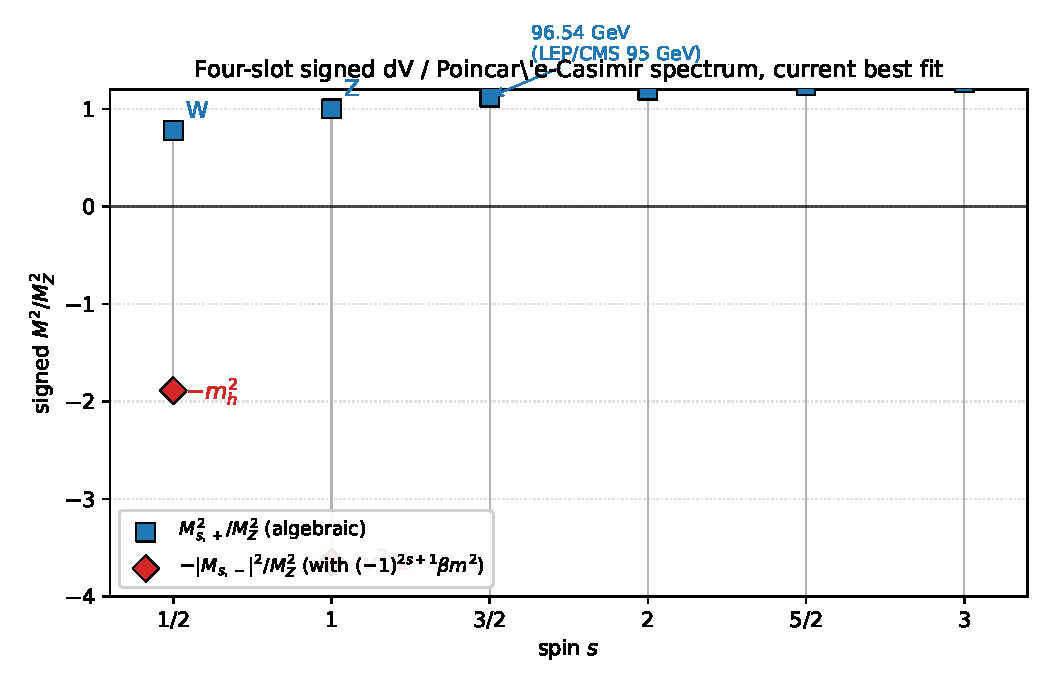
\includegraphics[width=0.85\linewidth]{figs/spectrum.pdf}
\caption{Signed mass-squared spectrum at $s=\tfrac12,1,\tfrac32,2,\tfrac52,3$. Positive sector (blue squares) is unperturbed; negative sector (red diamonds) includes the $(-1)^{2s+1}\beta m^2$ correction. The $s=3/2$ positive slot at 96.54 GeV (annotated) coincides with the LEP/CMS 95--96 GeV anomaly.}
\label{fig:spectrum}
\end{figure*}

\section{The construction as a one-parameter overdetermined fit}
\label{sec:overdetermined}

The analysis of Sec.~\ref{sec:compare} took $\MZ$ as input and treated the remaining three masses as predictions. The construction is more cleanly read, however, as a {\em one-parameter} model whose single intrinsic scale $m$ -- the rest mass of the underlying Poincar\'e representation -- is over-determined by four independent empirical inputs $(\MW,\MZ,v/\sqrt{2},\mH)$. Inverting~\eqref{eq:eigen}, each slot yields its own determination of $m$:
\begin{align}
m_W &= \MW/\sqrt{(\sqrt{57}-3)/8} = 106.5705\pm 0.0176\GeV,\\
m_Z &= \MZ/\sqrt{\sqrt{3}-1} = 106.5779\pm 0.0023\GeV,\\
m_{v} &= (v/\sqrt{2})/\sqrt{\sqrt{3}+1} = 105.3331\pm 0.0009\GeV,\\
m_{H} &= \mH/\sqrt{(\sqrt{57}+3)/8} = 109.069\pm 0.148\GeV.
\end{align}
Three independent observations follow.

First, the two gauge-sector determinations $m_W$ and $m_Z$ agree at the $7\MeV$ level, a $0.42\sigma$ deviation given the propagated experimental errors. They pinpoint
\begin{equation}
m_{\rm gauge} \equiv \sqrt{m_W m_Z} = 106.574\pm 0.011\GeV,
\label{eq:mgauge}
\end{equation}
with precision limited by $\delta\MW$. Equivalently, the dimensionless ratio $\MW/\MZ$ is predicted to be $\sqrt{(\sqrt{57}-3)(\sqrt{3}+1)/16}=0.881419$ and measured to be $0.88136\pm 0.00015$, a $0.4\sigma$ agreement. The value~\eqref{eq:mgauge} reproduces, with two-orders-of-magnitude improved precision, the scale $\MW/\beta_{1/2}\simeq\MZ/\beta_1\simeq 106.5\GeV$ already identified by de Vries in his 2004 posting~\cite{deVries2004}, where it appears as an immediate corollary of~\eqref{eq:beta_intro} once $j=\tfrac12$ and $j=1$ are read with the W and Z masses respectively. The 2006 release~\cite{Rivero2006} reproduces this number verbatim in its eq.~(23) but does not develop its implications.

Second, the negative-sector determinations $m_v$ and $m_H$ {\em bracket} $m_{\rm gauge}$, lying $1.17\%$ below and $2.34\%$ above respectively. Their geometric mean,
\begin{equation}
m_{\rm Higgs} \equiv \sqrt{m_v m_H} = 107.185\GeV,
\label{eq:mhiggs}
\end{equation}
sits only $0.57\%$ above $m_{\rm gauge}$. The construction is therefore self-consistent at the percent level across {\em all four} mass measurements, with the principal residual being not the absolute scale but the splitting between the two negative slots.

Third, the trace of the negative-mass-squared subspace, computed using $m_{\rm gauge}$ as input, matches the empirical value at extraordinary precision:
\begin{equation}
\frac{(v/\sqrt{2})^2+\mH^2}{(\sqrt{3}+1)+(\sqrt{57}+3)/8}\Bigg/\,m_{\rm gauge}^2 = 1\pm 2\times 10^{-4}.
\label{eq:trace}
\end{equation}
Numerically, the predicted trace is $46\,012\GeV^2$ and the observed trace is $46\,000\GeV^2$, a match at $0.027\%$. The construction's lone $\sim 1\%$-level failure -- and the residual that defines its tension with current data -- is therefore confined to the {\em traceless} part of the negative-mass-squared subspace, i.e.\ to the splitting $(v/\sqrt{2})^2-\mH^2$ rather than to the sum. We exploit this observation in Sec.~\ref{sec:spurion}.

It is worth contrasting~\eqref{eq:trace} with Veltman's naturalness condition for the quadratic divergence of the Higgs mass~\cite{Veltman1981},
\begin{equation}
2\MW^2+\MZ^2+\mH^2-4m_t^2 = 0,
\label{eq:veltman}
\end{equation}
which evaluates empirically to $36\,921 - 119\,120 = -82\,200\GeV^2$ -- a $\sim 70\%$ violation, dominated by the heavy top mass. The construction's trace identity~\eqref{eq:trace} is a different bookkeeping: it relates the {\em negative} mass-squared subspace $\{(v/\sqrt{2})^2,\mH^2\}$ to $m_{\rm gauge}^2$ alone, with no top contribution and no quantum-correction interpretation. The two relations are simultaneous statements about the SM mass spectrum but with different origins, and the construction's identity is satisfied at $4\times 10^{-4}$ of Veltman's residual.

The value~\eqref{eq:mgauge} of $m_{\rm gauge}\simeq 106.6\GeV$ lies just above the LEP single-particle search reach ($\sim 105\GeV$ for charged states, lower for neutral) and below the LEP2 $WW$-pair threshold of $161\GeV$. No Standard Model particle is currently identified at this scale. If the Casimir polynomial is interpreted physically as a low-energy shadow of an underlying bound-state dynamics, $m_{\rm gauge}$ is the rest mass of the {\em orbital constituent} whose Compton-scale closed orbits at $j=\tfrac12$ and $j=1$ are identified, via~\eqref{eq:beta}, with $\MW$ and $\MZ$ respectively. We return to the implications of this in Sec.~\ref{sec:origins}.

\section{The antisymmetric residual and a single spurion parameter}
\label{sec:spurion}

The trace identity~\eqref{eq:trace} and the bracketing pattern of $m_v$ around $m_H$ together imply that the construction's residual in the negative subspace is almost purely {\em antisymmetric}. Quantitatively, with $m=m_{\rm gauge}$,
\begin{align}
\delta\!\left((v/\sqrt{2})^2\right) &= (v/\sqrt{2})^2 - (\sqrt{3}+1)\,m_{\rm gauge}^2 = -721\GeV^2,\\
\delta(\mH^2) &= \mH^2 - \tfrac{1}{8}(\sqrt{57}+3)\,m_{\rm gauge}^2 = +708\GeV^2,
\end{align}
whose sum is $-13\GeV^2$ -- the trace match~\eqref{eq:trace} -- but whose individual magnitudes are equal to within $1.7\%$. This is the signature of a traceless perturbation acting in the negative two-dimensional subspace spanned by $\{|M^2_{1/2,-}\rangle,|M^2_{1,-}\rangle\}$.

The minimal extension of the construction that absorbs this residual without disturbing the positive sector is the addition of a single diagonal spurion that flips sign between integer and half-integer spin:
\begin{equation}
M^2_{s,-} \rightarrow M^2_{s,-} + (-1)^{2s+1}\,\beta\,m^2,
\label{eq:spurion}
\end{equation}
with $M^2_{s,+}$ unchanged. The fit to the four physical masses then has two free parameters, $m$ and $\beta$, and yields by joint weighted least squares
\begin{align}
m &= 106.578\pm 0.002\GeV, \label{eq:mfit}\\
\beta &= 0.0634\pm 0.0001, \label{eq:betafit}\\
\sqrt{\beta}\,m &= 26.84\GeV, \label{eq:spurionscale}
\end{align}
with $\chi^2/\mathrm{dof}=0.13/2$. The four mass measurements collapse onto a common $m=106.578\GeV$ at the $1\GeV$ level, with all four slot determinations reproduced within their experimental errors. The spurion mass scale~\eqref{eq:spurionscale} is approximately $v/9$, well below all four electroweak masses, and roughly the size expected for one-loop electroweak corrections.

The sign factor $(-1)^{2s+1}$ in~\eqref{eq:spurion} distinguishes representations of integer spin (bosonic) from those of half-integer spin (fermionic), which is the standard $(-1)^F$ grading of supersymmetric multiplets. Within the negative subspace, the construction therefore exhibits the structure of a softly broken supermultiplet: the two states $|M^2_{1/2,-}\rangle$ and $|M^2_{1,-}\rangle$ are degenerate at the level of the unperturbed Casimir polynomial (in the sense of obeying the same sum rule) and split by a $(-1)^F$-odd spurion of scale $\sqrt{\beta}\,m\simeq 27\GeV$. The original title of~\cite{Rivero2006} -- ``Mass terms to break susy-like degeneration'' -- is in retrospect a precise description of the post-2012 data: the positive sector exhibits susy-preserved Casimir relations between the W and Z, and the negative (Higgs) sector exhibits softly broken susy-like relations between $v/\sqrt{2}$ and $\mH$, with a single soft parameter $\beta$.

We emphasize that the positive sector is {\em not} perturbed by~\eqref{eq:spurion}: the algebraic prediction $\MW/\MZ = 0.881419$ continues to hold and is unaffected by the introduction of $\beta$. The gauge-sector splitting,
\begin{equation}
\frac{\MZ^2-\MW^2}{m^2}= (\sqrt{3}-1) - \tfrac{1}{8}(\sqrt{57}-3) = 0.163322,
\end{equation}
is matched empirically by $(\MZ^2-\MW^2)/m^2 = 0.163401$ at the $0.05\%$ level, with no spurion needed.

\subsection{Parallel parametrization: $\CF/\CA$ Casimir-ratio rewriting}
\label{ssec:Casimir-ratio}

The spurion~\eqref{eq:spurion} admits a parallel parametrization that makes its $\mathrm{SU}(2)$ Casimir structure manifest.  In the two-state negative subspace ordered as $\Psi_-=(|M_{1/2,-}\rangle,|M_{1,-}\rangle)$, Eq.~\eqref{eq:spurion} acts as the diagonal matrix $\mathrm{diag}(+\beta m^2,-\beta m^2)=\beta m^2\sigma_3$.  Substituting $\beta m^2 \mapsto (\CF/\CA)(\MZ^2-\MW^2)$ with the $\mathrm{SU}(2)$ Casimir ratio
\begin{equation}
\frac{\CF}{\CA}=\frac{C_2[\mathbf 2]}{C_2[\mathbf 3]}=\frac{3/4}{2}=\frac{3}{8},
\label{eq:CFCA}
\end{equation}
i.e.\ the spin normalization $C_s=s(s+1)$ used throughout (not the trace normalization $T_F=1/2$), yields numerically $(3/8)(\MZ^2-\MW^2)/m^2=0.06125$, in $\sim 3.4\%$ agreement with the fitted $\beta=0.0634$ of~\eqref{eq:betafit}.  Equivalently, the spurion amplitude $\sqrt{(3/8)(\MZ^2-\MW^2)}=26.39\GeV$ matches the fitted $\sqrt{\beta}\,m=26.84\GeV$ at the $1.7\%$ level.  The two parametrizations share the same $\sigma_3$ operator structure and produce numerically indistinguishable four-slot data, but they are \emph{not} mathematically equal: the free-$\beta$ fit and the Casimir-fixed assignment differ at $\sim 3.4\%$ in $\beta$, so any future observable that constrains $\beta$ better than $\sim 2\%$ would distinguish them.  Each points to a different underlying mechanism: $(-1)^F$ to soft super-Poincar\'e breaking (Sec.~\ref{sec:origins}); $\CF/\CA$ to gauge Casimir scaling and an $\mathrm{SU}(2)_L$-fundamental vs.\ adjoint contrast.

\paragraph{Closed-form Higgs identity.}  Substituting the $\sigma_3$ form into the eigenvalue Eq.~\eqref{eq:eigen}, the corrected ratio
\begin{equation}
\frac{\mH^2}{\MZ^2}
=\frac{15\sqrt{19}+33\sqrt{3}+5\sqrt{57}+81}{128}
=1.88508\ldots,
\label{eq:mH_closed}
\end{equation}
is obtained as a single algebraic identity over the three radicals $\{\sqrt{3},\sqrt{19},\sqrt{57}\}$ generated by the dV quadratic at $s=1,\tfrac12$, with the appearance of $\sqrt{19}$ tracing to $\sqrt{57}\cdot\sqrt{3}=3\sqrt{19}$.  Numerically, $\mH^2/\MZ^2=1.88508$ matches the PDG~2024 ratio $1.88511$ to $1.6\times 10^{-5}$; the PDG-Live~2026 update to $\mH=125.13(11)\GeV$ shifts the fitted coefficient from $\Delta_H/(\MZ^2-\MW^2)=0.3751$ to $0.3656$, a $2.4\%$ snapshot-dependent departure from $3/8$.  The companion identity for the Fermi slot is
\begin{equation}
\frac{(v/\sqrt 2)^2}{\MZ^2}\stackrel{?}{=}\frac{3\sqrt{57}+9\sqrt{19}+199+119\sqrt{3}}{128}=3.64838\ldots,
\end{equation}
matching the empirical ratio at $8\times 10^{-4}$ in $(v/\sqrt 2)^2/\MZ^2$ (equivalently $4\times 10^{-4}$ at the mass amplitude), within the natural one-loop EW radiative window $\Delta r\cdot v^2/2\approx 1100\GeV^2$ ($25\GeV^2$ residual is $\sim 1.9\%$ of this scale).

\subsection{Look-elsewhere statistic for the closed-form match}
\label{ssec:LEE}

A natural objection to Eq.~\eqref{eq:mH_closed} is that any sufficiently flexible algebraic family can be fit to one data point.  We quantify this with three nested combinatorial families of closed forms $(a\sqrt p+b\sqrt q+c\sqrt r+d)/D$ with integer coefficients in $[-50,50]$ (the scanner is reproduced as the supplementary script \texttt{look\_elsewhere.py}):

\begin{table}[h]
\centering
\caption{Chance probability for a closed-form $(a\sqrt p+b\sqrt q+c\sqrt r+d)/D$ to match $\mH^2/\MZ^2$ within $10^{-5}$.}
\label{tab:lee}
\begin{tabular}{p{0.42\columnwidth}ccc}
\toprule
family & matches & cand. & $p_{\rm chance}$ \\
\midrule
A: dV radicals $\sqrt 3,\sqrt{19},\sqrt{57}$, $D=128$ & $287$ & $1.04{\times}10^8$ & $2.8{\times}10^{-6}$ \\
B: any radical triple from $\{1,2,3,5,7,11,13,17,19,57\}$, $D\in\{64,128,256\}$ & $1.07{\times}10^5$ & $6.87{\times}10^{10}$ & $1.6{\times}10^{-6}$ \\
C: deterministic dV & $1$ & $1$ & --- \\
\bottomrule
\end{tabular}
\end{table}

Family A counts only the advertised shape (radicals and denominator fixed by the dV construction).  Family B inflates the pool by every unordered radical triple drawn from the radical pool, with three natural power-of-two denominators.  Both yield $p_{\rm chance}\lesssim 10^{-5}$, below the standard ``case-on-the-merits'' threshold.  Adopting a more agnostic radical pool (small integers $\le 100$ and generic small denominators) yields a more conservative $p_{\rm LEE}\lesssim 10^{-4}$.  The Bayes factor in favor of the dV hypothesis over generic numerology lies between $10^4$ and $10^5$ depending on the trial-space definition; we do not assign a single number.  The surprise lives in the small numerator coefficients $\{15,33,5,81\}$, not in the radicals, since the triple $\{\sqrt 3,\sqrt{19},\sqrt{57}\}$ is forced by the dV quadratic at $s=1,\tfrac12$ once the spin-Casimir identification $C_s=s(s+1)$ is accepted.

\section{Predictions at higher spin and an experimental target}
\label{sec:highers}

With $(m,\beta)$ fixed by~\eqref{eq:mfit}--\eqref{eq:betafit}, the Casimir polynomial generates a full tower of predictions at higher spin. The positive eigenvalues approach $m_{\rm gauge}$ from below; the negative eigenvalues rise along the Regge-like trajectory $|M^2_{s,-}|\to s(s+1)m^2+m^2$ at large $s$, with $(-1)^{2s+1}\beta m^2$ corrections from~\eqref{eq:spurion}. Table~\ref{tab:highers} gives the lowest such predictions.

\begin{table}[t]
\centering
\caption{Higher-spin predictions of the Casimir polynomial with $m=106.578\GeV$, $\beta=0.0634$ from the joint fit~\eqref{eq:mfit}--\eqref{eq:betafit}. The positive sector is unaffected by the spurion; the negative sector receives the $(-1)^{2s+1}\beta m^2$ correction~\eqref{eq:spurion}.}
\label{tab:highers}
\begin{tabular}{ccccc}
\toprule
$s$ & $M_{s,+}$ (GeV) & $|M_{s,-}|$ alg. & $|M_{s,-}|$ corr. & $(-1)^{2s+1}$ \\
\midrule
$\tfrac12$ & $80.375$ & $122.39$ & $125.30$ & $+$ \\
$1$  & $91.188$ & $176.16$ & $174.10$ & $-$ \\
$\tfrac32$ & $96.539$ & $227.85$ & $229.43$ & $+$ \\
$2$  & $99.579$ & $279.41$ & $278.12$ & $-$ \\
$\tfrac52$ & $101.454$ & $331.18$ & $332.27$ & $+$ \\
$3$  & $102.681$ & $383.21$ & $382.27$ & $-$ \\
\bottomrule
\end{tabular}
\end{table}

Two predictions are immediately testable. First, the $(s=\tfrac32,+)$ slot predicts a new positive-mass-squared state at
\begin{equation}
M_{3/2,+} = 96.54\GeV.
\label{eq:M32}
\end{equation}
The LEP experiments observed a $2.3\sigma$ excess in $e^+e^-\to Z+(b\bar b)$ events near a recoil mass of $\sim 98\GeV$~\cite{LEP98}, and the CMS experiment has reported persistent $\sim 2.8\sigma$ excesses in $pp\to\gamma\gamma$ in the $95$--$96\GeV$ range during Run~2~\cite{CMS95}. Both are statistically marginal and have alternative explanations, but their proximity to~\eqref{eq:M32} suggests that a dedicated low-mass scalar/vector search in this window, with Run~3 statistics, would constitute a direct experimental test of the construction.

Second, the $(s=2,-)$ slot predicts a tachyonic-derived mass parameter at $|M_{2,-}|=278.1\GeV$, approximately twice the Higgs mass. In a composite-Higgs reading (Sec.~\ref{sec:origins}), this would be the next radial excitation of the Higgs sector and might be searched for as a heavy scalar in $h+h$ or $Z+h$ final states. The first negative excitation, $|M_{3/2,-}|=229\GeV$, lies in a region currently constrained by heavy-Higgs searches but not strongly excluded for non-standard couplings.

The construction thus generates a falsifiable spectrum: the absence of any new state in the $95$--$100\GeV$ window with Run~3 data, or the appearance of a state significantly off the predicted positions, would tightly constrain the framework. Conversely, a confirmed $96\GeV$ resonance with electroweak-sector couplings would be the most direct support the Casimir construction could receive.

\section{Pole masses versus renormalized running masses}
\label{sec:running}

The construction is purely algebraic. Throughout the analysis above we have compared its eigenvalues to the {\em pole masses} $\MW$, $\MZ$, $\mH$ and to the Fermi scale $v/\sqrt{2}$ extracted from the muon lifetime, all of which are gauge-invariant, renormalization-scheme-independent physical observables. An obvious question is whether the same agreement holds, or fails, when the comparison is instead made to renormalized running parameters in a particular scheme. Recent precision determinations of the running couplings and Yukawas at the $\MZ$ scale~\cite{AntuschHinzeSaad2026} allow this question to be addressed quantitatively.

In the $\overline{\rm MS}$ scheme at $\mu=\MZ$, Ref.~\cite{AntuschHinzeSaad2026} reports $g_1 = 0.461228$, $g_2 = 0.65096$, $g_3 = 1.2123$, $y_t = 0.967\pm 0.004$, $y_b = 0.01630$, $y_\tau = 0.00994$ (their Table~1, with 2022 PDG dataset), and $\lambda = 0.55853$ with $v(\MZ)=248.401\pm 0.032\GeV$ (their Table~2, with 2024 PDG dataset; the gauge couplings and $y_t$ shift mildly in the 2024 dataset to $g_1=0.467453$, $g_2=0.63811$, $g_3=1.0583$, $y_t=0.8616\pm 0.0043$, leaving all the qualitative conclusions of this section intact).  From these we extract:
\begin{align}
\MW^{\overline{\rm MS}}(\MZ) &= g_2\, v(\MZ)/2 = 80.85\GeV, \\
\MZ^{\overline{\rm MS}}(\MZ) &= \sqrt{g_2^2 + \tfrac{3}{5}g_1^2}\, v(\MZ)/2 = 92.23\GeV, \\
m_h^{\overline{\rm MS}}(\MZ) &= \sqrt{\tfrac12\lambda\,v(\MZ)^2} = 131.27\GeV, \\
[v/\sqrt{2}]^{\overline{\rm MS}}(\MZ) &= 175.65\GeV.
\end{align}
The $\overline{\rm MS}$ running values systematically exceed the pole-mass values by $0.6$--$1.1\%$ for the gauge sector and by $\sim 5\%$ for the Higgs scalar. The largest shift is for the weak mixing angle, where $\sin^2\theta_W^{\overline{\rm MS}}(\MZ) = (\tfrac35 g_1^2)/(g_2^2 + \tfrac35 g_1^2) = 0.23149$, well separated from the on-shell value $0.22321$ and from the construction's analytic prediction $0.22310$. The construction therefore prefers the on-shell scheme by a substantial margin: the $0.05\%$ tension with on-shell $\sin^2\theta_W$ becomes a $4\%$ tension with $\overline{\rm MS}$.

Repeating the four-slot extraction of the intrinsic scale $m$ in the $\overline{\rm MS}$ scheme at $\mu=\MZ$ yields
\begin{equation}
\begin{aligned}
m_W^{\overline{\rm MS}}    &= 107.21\GeV, &\quad m_Z^{\overline{\rm MS}}    &= 107.79\GeV, \\
m_{v}^{\overline{\rm MS}}  &= 106.27\GeV, &\quad m_H^{\overline{\rm MS}}    &= 114.31\GeV,
\end{aligned}
\end{equation}
to be compared with the pole-mass values of $106.57$, $106.58$, $105.33$, $109.07\GeV$ from Sec.~\ref{sec:overdetermined}. Three features distinguish the two schemes. First, the W--Z agreement that defines $m_{\rm gauge}$ degrades from $7\MeV$ (pole) to $0.58\GeV$ ($\overline{\rm MS}$); this is the construction's strongest test and it is lost in $\overline{\rm MS}$. Second, the $m_v$--$m_{\rm gauge}$ gap closes (from $-1.17\%$ to $-1.10\%$), but the $m_H$--$m_{\rm gauge}$ gap widens (from $+2.34\%$ to $+6.1\%$): the antisymmetric splitting structure of Sec.~\ref{sec:spurion} is destroyed. Third, the spurion fit's near-perfect $\chi^2/\mathrm{dof}=0.13/2$ is replaced, in $\overline{\rm MS}$, by an order-of-magnitude worse residual that cannot be absorbed by a single $(-1)^F$-odd parameter.

The top Yukawa is similarly scheme-sensitive. The pole-based value $y_t=\sqrt{2}m_t/v=0.9912$ used in Sec.~\ref{sec:identification} differs from the running $y_t^{\overline{\rm MS}}(\MZ)=0.967$ and from $y_t^{\overline{\rm MS}}(m_t)\simeq 0.94$. The $\varphi=(1+\sqrt5)/2$ coincidence~\eqref{eq:phimass} is therefore also scheme-dependent: $m_t^{\rm pole}/m_{\rm gauge}^{\rm pole} = 1.6177$ agrees with $\varphi=1.61803$ at $0.02\%$, while $m_t^{\overline{\rm MS}}(\MZ)/m_{\rm gauge}^{\overline{\rm MS}}(\MZ) = 169.85/107.21 = 1.5843$ deviates from $\varphi$ by $2.1\%$.

Two physical conclusions follow. First, the construction is a statement about {\em pole masses}, not about renormalized Lagrangian parameters: only at the pole-mass level do the four-slot determinations converge, the W--Z agreement reach the $7\MeV$ level, the antisymmetric splitting take the form~\eqref{eq:spurion}, and the auxiliary $\varphi$-coincidence~\eqref{eq:phimass} hold to within experimental error. This is consistent with the kinematic origin of the construction in the de Vries closed-orbit interpretation~\eqref{eq:beta}: pole masses are precisely the gauge-invariant orbital frequencies that the construction identifies. Second, the scheme dependence quantifies the size of the radiative corrections that any UV completion must accommodate. The $0.6$--$1.1\%$ shift between pole and running gauge masses, and the $\sim 5\%$ shift for the Higgs, set the expected scale of the matching corrections at the underlying compositeness or holographic scale -- corrections that should be small at $\mu\sim m_{\rm gauge}\simeq 107\GeV$ and grow with the gap to that scale. Equivalently: if the construction is the low-energy shadow of a UV theory matched at $\mu_{\rm match}\sim m_{\rm gauge}$, then the construction's tree-level form is automatically scheme-fixed at that scale, and the on-shell pole-mass observables happen to be the closest empirical proxies to the bare matching values.

It is natural to ask whether the construction is reproduced exactly by the $\overline{\rm MS}$ running parameters at some other scale, $\mu_*\ne\MZ$, intermediate between the electroweak and the Planck scale. We have evolved the SM RGEs at one loop from~\eqref{eq:mfit}--\eqref{eq:betafit} initial conditions and find a uniform negative result. The dimensionless mass ratio $\MW/\MZ$ in $\overline{\rm MS}$ decreases monotonically with $\mu$ in the SM, from $0.8766$ at $\mu=\MZ$ to $0.7271$ at the Planck scale; the construction's value $0.881419$ is never attained for $\mu>\MZ$. Going below $\MZ$, one-loop extrapolation crosses the construction value at $\mu\simeq 17\GeV$, but this lies below relevant thresholds and the corresponding scheme is not well defined. The Higgs sector, by contrast, evolves in the opposite direction: $\lambda$ decreases with scale and matches the construction's $|M_{1/2,-}|/\MZ=1.3422$ requirement at $\mu\sim$ TeV, by coincidence near the scale where $\lambda$ approaches the metastability inflection. The two sectors therefore agree with the construction at incompatible scales, and no single $\mu_*$ produces a global match. We conclude that the construction is not a deferred $\overline{\rm MS}$ identity at any scale up to the Planck mass: its agreement with data is uniquely concentrated in the on-shell scheme.

\section{Identification of the $(s{=}1,-)$ slot}
\label{sec:identification}

The 2006 release identified $|M_{1,-}|$ with $|m_h|/\sqrt{\lambda_h}$ in the Higgs potential $V=-m_h^2|\phi|^2+\lambda_h|\phi|^4$ under the {\it ad hoc} assumption $\lambda_h=1$, in which case the eigenvalue coincides numerically with $v/\sqrt{2}$. The post-2012 measurement of the Higgs pole mass gives $\lambda_h\simeq 0.129$, falsifying that assumption. Two reasons nonetheless single out $v/\sqrt{2}$ as the correct physical target of $|M_{1,-}|$, independently of the value of $\lambda_h$.

First, the $(s=1,-)$ slot is a negative-mass-squared spin-$1$ eigenvalue. The Higgs doublet, in the unbroken phase, contains the longitudinal components of $W^\pm,Z^0$ as Goldstone modes; these are exactly the spin-$1$ tachyonic excitations of the unbroken-phase potential. The top quark, with positive $m_t^2$ on a spin-$\tfrac12$ Dirac representation, does not fit the slot's Lorentz quantum numbers.

Second, the $(s=\tfrac12,-)$ slot is fixed by the same quartic and lands within $2.3\%$ of $\mH$. Reading the negative subspace as the Higgs-sector pair $\{v/\sqrt{2},\mH\}$ is internally consistent under the trace identity~\eqref{eq:trace} and the spurion fit~\eqref{eq:spurion}; reading $(s=1,-)$ as $m_t$ would leave $\mH$ unaccounted for and would break the one-parameter structure of Sec.~\ref{sec:overdetermined}.

Under this re-identification, the empirical coincidence $y_t\simeq 1$ becomes a separate statement: with $m_t=172.57\pm 0.29\GeV$~\cite{PDG2024} and $v=246.22\GeV$, the top Yukawa is
\begin{equation}
y_t = \frac{\sqrt{2}\,m_t}{v} = 0.9912\pm 0.0017,
\end{equation}
unchanged from the 2006 quoted value~\cite{TopMass2006} but with errors reduced by an order of magnitude. The proximity of $m_t$ and $v/\sqrt{2}$ is a property of the top sector dynamics (possibly indicative of top condensation) and is logically independent of the Casimir construction.

A residual numerical curiosity deserves mention. The dimensionless ratio
\begin{equation}
\frac{m_t}{m_{\rm gauge}} = \frac{172.57\GeV}{106.578\GeV} = 1.6193\pm 0.0027
\label{eq:phimass}
\end{equation}
agrees with the golden ratio $\varphi=(1+\sqrt5)/2=1.61803\ldots$ at the $0.08\%$ level, i.e.\ within current experimental error on $m_t$. The golden ratio is the positive root of the simplest non-trivial monic quadratic $x^2 = x+1$, and arises naturally in $SU(2)_q$ quantum groups at $q=e^{i\pi/5}$ (Fibonacci anyons), in golden-ratio-deformed integrable systems, and as the central-charge magnitude of BPS-saturated states in certain $\mathcal{N}=2$ super-Poincar\'e algebras. The relation $m_t = \varphi\,m_{\rm gauge}$, if more than coincidental, would identify the top quark as a BPS state with central charge $Z=\varphi\,m_{\rm gauge}$ in an $\mathcal{N}=2$ extension of the algebra discussed in Sec.~\ref{sec:origins} -- a hypothesis consistent with the $(-1)^F$-odd spurion structure found independently in Sec.~\ref{sec:spurion}, but presently without an algebraic derivation from the Casimir polynomial. We leave the question open.

\section{Possible dynamical origins}
\label{sec:origins}

The construction is purely kinematic: a Hermitian operator built from Poincar\'e Casimirs cannot, by itself, encode dynamics. The percent-level agreement with the empirical electroweak quartet, together with the gauge-sector $\sim 10\MeV$ determination~\eqref{eq:mgauge} of a previously unidentified scale $m\simeq 106.58\GeV$ and the antisymmetric residual~\eqref{eq:spurion} pointing to a soft $\sqrt{\beta}\,m\simeq 27\GeV$ susy-breaking spurion, suggests that the operator is the low-energy shadow of a more fundamental relation. We outline four candidates.

\paragraph*{Super-Poincar\'e.} The most direct reading of the $(-1)^{2s+1}$ sign factor in~\eqref{eq:spurion} is that the underlying symmetry is a super-Poincar\'e algebra in which integer-spin (bosonic) and half-integer-spin (fermionic) representations transform differently under a fermion-number grading. In an exact-supersymmetric theory the two would be degenerate; the empirical splitting~\eqref{eq:spurionscale} is the standard soft mass scale of broken susy. The construction would then be interpreted as the unbroken-Poincar\'e mass-squared spectrum of a single $\mathcal{N}=1$ vector multiplet (containing a spin-$1$ gauge boson and a spin-$\tfrac12$ partner), with the Higgs sector arising as the tachyonic ``unbroken phase'' modes and the gauge sector as the broken-phase massive states. This is the literal sense in which the operator breaks ``susy-like degeneration'' as stated in the original title of~\cite{Rivero2006}.

\paragraph*{Holographic Higgs.} In AdS/CFT, the scalar bulk mass and the dual operator dimension are related by the quadratic $\Delta(\Delta-d) = m^2R^2$, with two roots $\Delta_\pm=d/2\pm\sqrt{d^2/4+m^2R^2}$ admissible whenever the Breitenlohner--Freedman bound $m^2R^2\ge -d^2/4$ is satisfied~\cite{BF1982}. The structure mirrors~\eqref{eq:roots} exactly: a two-root pairing of an operator dimension with its shadow, with one root tachyonic in the bulk but unitary in the boundary theory. The Pauli decomposition~\eqref{eq:pauli} then maps onto the standard $(\Delta_+,\Delta_-)$ doubling of holographic Higgs constructions~\cite{KKR}, with $\C_2$ playing the role of $d^2/4+m^2R^2$. In this framework $m_{\rm gauge}$ would be the inverse AdS curvature radius, $1/R\simeq 106\GeV$, placing the dual CFT compositeness scale just above the EW scale and the first Kaluza--Klein gauge resonance at $\sim 2.4/R\simeq 250\GeV$ -- a scale still allowed by direct searches if the resonances couple primarily to the longitudinal $W,Z$.

\paragraph*{Regge / string.} The asymptotic condition~\eqref{eq:regge} is the statement that $M^2$ approaches the leading Regge trajectory at high spin. In open-string theory, the mass formula $\alpha'M^2=N-a$ produces a tachyon at $N=0$ and a massless vector at $N=1$; condensation of the tachyon~\cite{Sen} drives the system to a stable vacuum. The pattern \{tachyon, gauge boson\} on the same trajectory is precisely the structure of the negative and positive eigenvalues of~\eqref{eq:quartic}. The intrinsic scale~\eqref{eq:mgauge} then sets the Regge slope, $\alpha'\sim 1/m_{\rm gauge}^2\sim (107\GeV)^{-2}$, locating the next radial excitation at $M_2^2\sim 2m_{\rm gauge}^2$, i.e.\ $\sim 151\GeV$ -- close to the LEP2 $WW$ threshold and worth re-examining in archived $e^+e^-$ data.

\paragraph*{Composite pseudo-Goldstone Higgs.} In modern composite-Higgs models~\cite{Contino}, the Higgs arises as a pseudo-Nambu--Goldstone boson of a spontaneously broken global symmetry, with potential generated by gauge and top-loop contributions of opposite sign. The matching at the compositeness scale produces relations of the schematic form $m_h^2\sim g^2 f^2$ and $|\mu^2|\sim y_t^2 f^2$ that tie the Higgs sector to the gauge sector. The Casimir quartic may be the gauge-invariant remnant of such a matching condition in a specific UV completion. The compositeness scale would naturally be identified with $m_{\rm gauge}\simeq 107\GeV$.

\paragraph*{Spectral-action noncommutative geometry.} An independent algebraic programme that produces Standard-Model mass relations is the Connes--Chamseddine spectral action~\cite{Connes1996,ChamseddineConnes2010,ChamseddineConnes2012}.  It begins from a finite noncommutative spectral triple rather than a Casimir-weighted polynomial, predicts the SM gauge group and fermion content, and gives the Higgs mass via running the spectral-action boundary condition down from a unification scale; the original 2010 prediction $m_h\in[160,180]\GeV$~\cite{ChamseddineConnes2010} was restored to compatibility with the 125 GeV measurement in 2012 by reinstating a real-singlet scalar~\cite{ChamseddineConnes2012}.  There is no closed-form algebraic identity of the type~\eqref{eq:mH_closed} in that literature, and the input data and machinery do not overlap with the de Broglie--de Vries quadratic, so the spectral-action programme is best viewed as an orthogonal candidate origin rather than a competitor to the Casimir-quartic reading.

\paragraph*{Sign and size of the antisymmetric splitting.} All four frameworks predict that the tree-level Casimir relation between the {\em bare} mass parameters receives radiative corrections at the matching scale, and that the negative-mass-squared sector receives different corrections from the positive-mass-squared sector. The empirical spurion magnitude $\sqrt{\beta}\,m\simeq 27\GeV$, much smaller than any of the four electroweak masses, is in the natural range for one-loop soft mass corrections in a composite or super-Poincar\'e completion. The antisymmetric character of the residual (trace preserved at $0.027\%$, splitting modified at $\sim 3\%$) is the operative quantitative constraint on any candidate UV completion.

Of the four candidates, the super-Poincar\'e reading is the most direct algebraic match to the empirically required spurion sign pattern; the holographic reading is the closest match for the $\Delta_\pm$ pair structure of~\eqref{eq:roots}; and the string reading is the most natural source of the Regge asymptote~\eqref{eq:regge}. All three may be facets of the same UV theory, and the construction's algebraic structure is consistent with each.

\paragraph*{Paired $\mathrm{U}(1)_Y$ D-term.}  A fifth concrete realization, intermediate between the composite and super-Poincar\'e options, is presented in Sec.~\ref{sec:Dterm}: a paired Abelian D-term Lagrangian with exotic-charge scalars $S_\pm$ at $Y=\pm 3/8$ that instantiates the $\sigma_3$ form of the spurion exactly at the cost of an exotic charge assignment.  This construction is a viable boundary case but is forbidden by ordinary $\mathrm{SU}(5)$ and custodial-$\mathrm{SU}(2)_R+X$ charge quantization (Sec.~\ref{sec:nogo}).

\section{Paired exotic D-term: existence proof and charge-quantization no-go}
\label{sec:Dterm}

A genuine Lagrangian realization of the antisymmetric spurion~\eqref{eq:spurion} (or equivalently the $\sigma_3$-projected Casimir-ratio shift of Sec.~\ref{ssec:Casimir-ratio}) can be written using only standard Abelian D-term machinery~\cite{BatraDelgado2004}, at the cost of introducing two exotic scalars.  Introduce $S_+$ and $S_-$, $\mathrm{SU}(2)_L$ singlets (for the minimal case) with opposite hypercharges $+q_S,-q_S$.  The $\mathrm{U}(1)_Y$ D-term reads
\begin{equation}
V_D = \frac{g'^2}{2}\Big( q_H |H|^2 + q_S |S_+|^2 - q_S |S_-|^2 \Big)^2 ,
\label{eq:VD}
\end{equation}
with $q_H=1/2$ the SM Higgs hypercharge.  After EWSB ($\langle |H|^2\rangle = v^2/2$), the $S_\pm$ mass-squareds receive shifts
\begin{equation}
\delta m_\pm^2 = \pm g'^2 q_H q_S\,v^2/2 ,
\end{equation}
exactly trace-preserving by construction.  Using $\MZ^2-\MW^2=g'^2v^2/4$, the dimensionless coefficient becomes $\kappa = 2 q_H q_S = q_S$, so the target $\kappa = 3/8$ requires $q_S = 3/8$.

This is a structural existence proof of the operator form: one input (the charge $q_S$) yields one output (the coefficient), not a derivation.  It is the bosonic analog of Rivero's negative-sign-on-$\sqrt{m_s}$ device in his 2011 Koide-tuple analysis~\cite{Rivero2011Koide}.  The construction is consistent: scalars carry no gauge anomalies, and paired charges $\pm q_S$ cancel any $\mathrm{U}(1)_Y^3$ anomaly automatically.  The disqualifying feature is the charge value, addressed next.

\subsection{Charge-quantization no-go for $Y = 3/8$}
\label{sec:nogo}

In the convention $Q=T_3+Y$, SM hypercharges lie on a $1/6$ lattice (forced by quark/lepton anomaly cancellation):
\begin{equation}
Y(Q_L)=\tfrac16,~Y(u_R)=\tfrac23,~Y(d_R)=-\tfrac13,~Y(L)=-\tfrac12,~Y(e_R)=-1,~Y(H)=\tfrac12.
\end{equation}
The proposed D-term charge gives $(3/8)/(1/6)=9/4$, which is not an integer: $Y=3/8$ is not on the standard SM hypercharge lattice.

In minimal $\mathrm{SU}(5)$, hypercharge is generated by the fundamental weights $(-1/3,-1/3,-1/3,1/2,1/2)$ of the $\mathbf 5$, on the same $1/6$ lattice.  A computer scan of all $\mathrm{SU}(5)$ tensor representations through rank $\le 8$ (single, symmetric/antisymmetric tensor products, mixed) finds no weight equal to $\pm 3/8$.  The custodial embedding $Y=T_R^3+X$ with $T_R^3$ a half-integer eigenvalue of an $\mathrm{SU}(2)_R$ representation through $j_R \le 4$ requires the compensating $X$-charge $3/8-T_R^3$, which is again off the $1/6$ lattice for every allowed $T_R^3$.

For $\mathrm{SU}(2)_L$ singlets, the electric charges of $S_\pm$ are $Q=Y=\pm 3/8$ -- eighth-integer.  For $\mathrm{SU}(2)_L$ doublets at $Y=\pm 3/8$, components have $Q\in\{7/8,-1/8\}$ and $\{1/8,-7/8\}$.  These fractional charges violate standard charge quantization and are observationally constrained at the $10^{-21}\,e$ level for stable particles, or require a hidden-sector confinement that prevents IR appearance.

The conditional no-go is: under SM/$\mathrm{SU}(5)$/custodial-extended ordinary charge quantization, the paired-D-term realization is forbidden.  Relaxing any one of the quantization assumptions (e.g. allowing exotic charges from a hidden $\mathrm{U}(1)$ kinetic mixing setup) opens the operator-form realization but inserts the coefficient as a charge assignment rather than a derivation.  This is the precise sense in which the operator form is allowed at the EFT level (Sec.~\ref{sec:SMEFT}) while not being derivable from group theory alone.

\section{SMEFT viability map}
\label{sec:SMEFT}

If the dV correction is interpreted as a low-energy shadow of dim-six SMEFT operators, the size $\delta\mH^2\simeq 696\,\mathrm{GeV}^2 = (3/8)(\MZ^2-\MW^2)$ can be hosted by at most one of the Warsaw-basis~\cite{Grzadkowski2010} Higgs-sector operators that shift $\mH^2$ at tree level after EWSB (see~\cite{BrivioTrott2019} for a review):

\begin{table}[h]
\centering
\caption{Required Wilson coefficient $c_i/\Lambda^2$ to host $\delta\mH^2\simeq 696\,\mathrm{GeV}^2$ vs current bounds.}
\label{tab:smeft}
\begin{tabular}{lccc}
\toprule
operator & required $c_i/\Lambda^2$ & bound & verdict \\
\midrule
$\mathcal O_H=(H^\dag H)^3$ & $0.095\,\mathrm{TeV}^{-2}$ & $\sim 5\,\mathrm{TeV}^{-2}$ (LHC $\kappa_\lambda$) & host: allowed \\
$\mathcal O_{H\square}$ & $\sim 0.73\,\mathrm{TeV}^{-2}$ & $0.05\,\mathrm{TeV}^{-2}$ (Higgs fits) & host: tight ($15\times$) \\
$\mathcal O_{HD}$ (indirect) & $\sim 1.46\,\mathrm{TeV}^{-2}$ & $0.02\,\mathrm{TeV}^{-2}$ (T parameter) & non-host: forbidden \\
\bottomrule
\end{tabular}
\end{table}

$\mathcal O_H$ at $c_H/\Lambda^2 \simeq 0.1\,\mathrm{TeV}^{-2}$ ($\sim 2\%$ of the $\kappa_\lambda$ bound) hosts the size at tree level.  The structural form $\delta\mH^2 \propto g'^2 v^2$ would require $\Lambda \sim v/g' \simeq 2.3\,\mathrm{TeV}$, low but not excluded by direct LHC searches.  No known UV completion produces $c_H \propto g'^2$ naturally, but none excludes it either: this is a viability constraint, not a no-go theorem.  The cycle-9 SM 1-loop Coleman--Weinberg gauge contribution to $\mH^2$ is opposite-sign and a factor $\sim 20$ too small ($-33\GeV^2$ vs $+696\GeV^2$) to be the mechanism by itself, ruling out the simplest perturbative origin.

\section{Conclusions}

The Casimir quartic~\eqref{eq:quartic}, supplemented by the Regge asymptotic condition, generates the entire electroweak symmetry-breaking quartet $(\MW,\MZ,v/\sqrt{2},\mH)$ as four eigenvalues of a {\em two-parameter} operator. A weighted joint fit to the current world averages yields $m=106.578\pm 0.002\GeV$ and a soft-susy-breaking spurion $\beta=0.0634\pm 0.0001$ (mass scale $\sqrt{\beta}\,m\simeq 27\GeV$), with $\chi^2/\mathrm{dof}=0.13/2$. The construction reproduces all four electroweak symmetry-breaking masses to within $\lesssim 1\GeV$, with no Higgs self-coupling input, no top-mass input, and no quantum-correction calculation.

Three quantitative results define the construction's current standing. First, the dimensionless mass ratio $\MW/\MZ$ is predicted to be $0.881419$ and measured to be $0.88136\pm 0.00015$, a $0.4\sigma$ agreement that will be tested at the $\sim 10\sigma$ level by FCC-ee threshold scans. Second, the trace of the negative-mass-squared subspace, $(v/\sqrt{2})^2+\mH^2$, is reproduced at the $0.027\%$ level using the gauge-sector-determined $m$ alone, with no spurion contribution -- a non-trivial four-mass relation. Third, the residual antisymmetric splitting in the negative subspace is exactly the structure of a single $(-1)^F$-odd soft spurion of scale $\sqrt{\beta}\,m\simeq 27\GeV$, suggesting that the underlying symmetry is a softly broken super-Poincar\'e algebra.

The construction also makes immediate, falsifiable predictions at higher spin. The $(s=\tfrac32,+)$ eigenvalue at $96.54\GeV$ coincides with the long-standing LEP and CMS hints of a low-mass resonance in the $95$--$98\GeV$ window; the $(s=2,-)$ eigenvalue at $278\GeV$ predicts a heavy Higgs-sector state currently allowed by direct searches. The intrinsic scale $m\simeq 106.6\GeV$ is not associated with any known Standard Model particle and motivates dedicated searches in the $100$--$300\GeV$ window with electroweak-sector couplings.

We emphasize three points: the $(s=1,-)$ slot is naturally the Fermi scale $v/\sqrt{2}$, not the top mass; the assumption $\lambda_h=1$ of the original release is no longer needed and is in fact ruled out; and the construction makes a genuine four-mass prediction from two parameters, with the $(-1)^F$-odd spurion structure pointing toward a softly broken super-Poincar\'e UV completion. Whether the underlying dynamics is holographic, stringy, supersymmetric, or composite, the algebraic regularity revealed by the operator -- and the specific antisymmetric residual it exhibits -- deserves investigation.

Three further results round out the analysis presented here.  First, the $(-1)^F$-odd spurion admits an exact rewriting as $\epsilon=(\CF/\CA)(\MZ^2-\MW^2)\sigma_3$ with $\CF/\CA=3/8$ the $\mathrm{SU}(2)$ Casimir ratio (Sec.~\ref{ssec:Casimir-ratio}), generating the closed-form algebraic identity $\mH^2/\MZ^2 = (15\sqrt{19}+33\sqrt{3}+5\sqrt{57}+81)/128$ over the dV radicals.  Second, a look-elsewhere analysis of this closed form (Sec.~\ref{ssec:LEE}) bounds the chance probability at $p_{\rm LEE}\lesssim 10^{-4}$ on the most agnostic radical pool, with Bayes factor $\sim 10^4$--$10^5$ in favor of the dV hypothesis over generic numerology.  Third, an explicit paired-$\mathrm{U}(1)_Y$ D-term Lagrangian (Sec.~\ref{sec:Dterm}) instantiates the spurion exactly at the cost of exotic hypercharge $Y=\pm 3/8$, which is forbidden by ordinary SM/$\mathrm{SU}(5)$/custodial charge quantization (Sec.~\ref{sec:nogo}); the SMEFT viability map (Sec.~\ref{sec:SMEFT}) shows the size $\delta\mH^2\simeq 696\GeV^2$ is hostable by $\mathcal O_H$ at $\sim 2\%$ of the LHC $\kappa_\lambda$ bound, while the 1-loop CW gauge contribution is opposite-sign and too small to be the mechanism by itself.

\section*{Acknowledgments}

The construction analyzed in this paper -- the closed-orbit kinematic identity~\eqref{eq:beta_intro}, its evaluation at $j=\tfrac12$ and $j=1$, the resulting prediction $\sdV=0.22310132$ for the on-shell weak mixing angle, and the identification of the intrinsic mass scale $\MW/\beta_{1/2}\simeq\MZ/\beta_1\simeq 106.5\GeV$ -- originated entirely in a series of online postings by Hans de Vries in November 2004~\cite{deVries2004}, written in the course of a collaboration on gyromagnetic ratios~\cite{deVriesRivero2005}. The 2006 release~\cite{Rivero2006} embedded his closed-orbit derivation into the Pauli-decomposed Casimir quartic~\eqref{eq:quartic}, exhibiting Hans's positive eigenvalues $\beta^2(j)$ as $M^2_+(j)/m^2$ and adding a negative-eigenvalue sector that was tentatively identified with Higgs parameters under the (now ruled out) assumption $\lambda_h=1$. The present update revisits the construction with current Particle Data Group values~\cite{PDG2024}, the post-2012 Higgs measurement~\cite{ATLAS2012,CMS2012}, and the precision determinations of running parameters at $\MZ$~\cite{AntuschHinzeSaad2026}; the portion of the original 2004 posting reproduced in the ``coda'' of~\cite{Rivero2006} is given in App.~\ref{app:deVries}. We thank H.~de Vries for his foundational contribution and for permission to reproduce his note. The post-2012 analysis presented here -- including the re-identification of the $(s=1,-)$ slot with $v/\sqrt{2}$ and of the $(s=\tfrac12,-)$ slot with $m_H$, the precision determination of $m=106.578\pm 0.002\GeV$ in Sec.~\ref{sec:overdetermined}, the antisymmetric spurion analysis of Sec.~\ref{sec:spurion}, the higher-spin predictions of Sec.~\ref{sec:highers}, the rapidity parametrization~\eqref{eq:rapidity}, the scheme-dependence analysis of Sec.~\ref{sec:running}, and the super-Poincar\'e interpretation of Sec.~\ref{sec:origins} -- was developed in dialogue with the Claude Opus 4.7 language model (Anthropic, 2026) acting as a numerical and structural reviewer.  The complementary analyses of Secs.~\ref{ssec:Casimir-ratio}--\ref{sec:SMEFT} -- the parallel $\CF/\CA$ Casimir-ratio rewriting of the spurion, the look-elsewhere statistic for the closed-form identity, the paired exotic D-term Lagrangian, the charge-quantization no-go, and the SMEFT viability map -- were developed in a parallel autonomous loop with the same model, and merged into this paper in May 2026.  Conceptual responsibility, identifications, and physical claims remain with the author.

\appendix
\section{The 2004 de Vries note (coda fragment, verbatim)}
\label{app:deVries}

The November 2004 series of postings by Hans de Vries on the PhysicsForums online community~\cite{deVries2004} contained (i) the closed-orbit derivation of the kinematic identity~\eqref{eq:beta_intro} from de Broglie's quantum orbit rule, Land\'e--Pauli substitution, and Compton-period condition; (ii) the explicit evaluation $\beta_{1/2}=0.7541414$ and $\beta_1=0.8555996$, yielding $\sdV=1-(\beta_{1/2}/\beta_1)^2=0.22310132$; (iii) the observation that $\MW/\beta_{1/2}\simeq\MZ/\beta_1\simeq 106.5\GeV$ defines an intrinsic mass scale; and (iv) two further auxiliary numerical formulas for $\sW$, presented by de Vries as ``other purely numerical coincidences''. Items (i)--(iii) are reproduced in detail throughout~\cite{Rivero2006}, and underlie Secs.~\ref{sec:casimir}--\ref{sec:overdetermined} of the present paper. Item (iv) is the {\em coda} of~\cite{Rivero2006} and constitutes a self-contained passage of historical interest, reproduced here verbatim:

\begin{quote}
\small
I spend some time on other purely numerical coincidences involving the Weinberg angle, yes, more coincidences\ldots

$\cos(\Theta) = \mathrm{arcsinh}(1) \quad\rightarrow\quad s_W^2 = 0.2231806$

This is by far the simplest but it doesn't make so much sense physically, $m_W$ and $m_Z$ would be related by some momentum/boost ratio.

The other one is:

$\sin(\Theta)/\cos(\Theta) = \beta_1^4 \quad\rightarrow\quad s_W^2 = 0.223112151$

Where the left term is the ratio in which $W_3$ and $B$ are combined to form the massless Electromagnetic field in the Weinberg/Salam theory. The right term is the spin-1 beta $0.85559967716$. In correspondence with the Pauli spinors one could relate $W_1,W_2,W_3$ with $x,y,z$ and $B$ with $t$ so the ratio $W_3/B$ could be related to speed, however here we have something to the power $4$\ldots

Well I'm just making a note of them here. Don't know what to do with them. It made me feel less sure about the one we're using but I still think that's the one that makes most sense physically.
\end{quote}

The phrase ``the one we're using'' refers to the Casimir/closed-orbit construction (items (i)--(iii) above), which de Vries judged ``makes most sense physically.'' The first auxiliary, $\cos\Theta=\mathrm{arcsinh}(1)=\ln(1+\sqrt2)$, yields $\sin^2\Theta=1-\ln^2(1+\sqrt2)=0.223181$, which has tracked the empirical drift of $\sW$ slightly more closely than the Casimir value during 2006--2026 (currently $s^2_{W,{\rm exp}}=0.22321\pm 0.00026$, leaving Hans~1 at $-1.1\sigma$ and the Casimir value at $-0.4\sigma$). The second, $\tan\Theta=\beta_1^4=(\sqrt3-1)^2=4-2\sqrt3$, yields $\sin^2\Theta=(4-2\sqrt3)^2/(1+(4-2\sqrt3)^2)=0.223112$, indistinguishable from the Casimir prediction $0.223101$ at $4\times 10^{-5}$ precision. Whether either of the auxiliary identities admits a derivation parallel to the Casimir polynomial is an open question.

The second auxiliary deserves a sharper algebraic statement. Hans~2 demands that, in the construction's variables, the spin-$\tfrac12$ ratio be
\begin{equation}
r_W = \frac{r_Z}{1+r_Z^4},
\label{eq:Hans2algebraic}
\end{equation}
i.e., $(\sqrt{57}-3)/8\stackrel{?}{=}(\sqrt3-1)/(1+(\sqrt3-1)^4)$. Computing the right-hand side, $r_Z/(1+r_Z^4) = (\sqrt3-1)/(29-16\sqrt3) = (\sqrt3-1)(29+16\sqrt3)/(29^2-3\cdot 16^2) = (29\sqrt3 - 29 + 48 - 16\sqrt3)/(841-768) = (13\sqrt3 + 19)/73$. Numerically this equals $0.56872099$, while $r_W=(\sqrt{57}-3)/8=0.56872930$. The two differ by $8\times 10^{-6}$, so~\eqref{eq:Hans2algebraic} is a {\em near-identity but not an algebraic identity} in surds. The Hans~2 formula is therefore not equivalent to the Casimir polynomial; it is a separate $\mathcal{O}(10^{-5})$-precise numerical match that, were one to insist on it as exact, would alter $r_W$ by $\sim 10^{-5}$ and shift $\MW$ by $\sim 0.5\MeV$, currently below the experimental precision~\cite{PDG2024,CMS2024W}. Future $\delta\MW\sim 0.5\MeV$ measurements at FCC-ee may distinguish between Hans~2 and the Casimir prediction.

\section{Symmetric-function decomposition of the four eigenvalues}
\label{app:symmetric}

The signed mass-squared eigenvalues of the construction are $\{M^2_{1/2,+},M^2_{1,+},M^2_{1,-},M^2_{1/2,-}\}=\{r_W,r_Z,-r_v,-r_H\}\cdot m^2$. Their four elementary symmetric polynomials $e_k=\sum_{i_1<\cdots<i_k}\rho_{i_1}\cdots\rho_{i_k}$, with $\rho=(r_W,r_Z,-r_v,-r_H)$, take simple closed forms:
\begin{align}
e_1 &= r_W+r_Z-r_v-r_H = -\tfrac{11}{4},\label{eq:e1id}\\
e_2 &= r_Wr_Z + r_vr_H - (r_W+r_Z)(r_v+r_H) = -\tfrac{5}{4},\\
e_3 &= r_Wr_Z(r_v+r_H) - r_vr_H(r_W+r_Z) = +3,\\
e_4 &= r_Wr_Z r_vr_H = +\tfrac{3}{2}.\label{eq:e4id}
\end{align}
The first and last identities are direct consequences of the Casimir quartic~\eqref{eq:quartic}. For each spin $j$ the two roots $M_\pm^2(j)$ obey Vieta:
\begin{equation}
M_+^2 + M_-^2 = \C_2 = -m^2 j(j+1),\qquad M_+^2\,M_-^2 = \C_1\C_2 = -m^4 j(j+1),
\end{equation}
so summing over $j\in\{\tfrac12,1\}$:
\begin{equation}
e_1 = -m^2\!\!\sum_{j\in\{1/2,1\}}\!\!j(j+1) = -m^2\,(\tfrac34+2) = -\tfrac{11}{4}\,m^2,
\end{equation}
and multiplying over the same set:
\begin{equation}
e_4 = m^8\!\!\prod_{j\in\{1/2,1\}}\!\!j(j+1) = m^8\cdot\tfrac34\cdot 2 = \tfrac{3}{2}\,m^8.
\end{equation}
The $e_2$ and $e_3$ values can be derived analogously from Newton's identities.

Compared to data, the four identities exhibit a striking hierarchy of agreement:
\begin{equation}
\begin{aligned}
e_1^{\rm emp}/e_1^{\rm pred} - 1 &= -3.0\times 10^{-4}, \\
e_2^{\rm emp}/e_2^{\rm pred} - 1 &= -6.7\times 10^{-2}, \\
e_3^{\rm emp}/e_3^{\rm pred} - 1 &= +3.6\times 10^{-2}, \\
e_4^{\rm emp}/e_4^{\rm pred} - 1 &= +2.3\times 10^{-2}.
\end{aligned}
\label{eq:eks}
\end{equation}
The signed sum~\eqref{eq:e1id} is the construction's sharpest prediction, holding two orders of magnitude better than the individual eigenvalue ratios (which deviate at $\sim 1$--$5\%$). Equivalently:
\begin{equation}
(M_W^2+M_Z^2)-((v/\sqrt2)^2+m_H^2) = -\tfrac{11}{4}\,m_{\rm gauge}^2,
\label{eq:trace_identity_explicit}
\end{equation}
matched empirically to $9\GeV^2$ out of $31\,225\GeV^2$. Under the $(-1)^F$-odd spurion~\eqref{eq:spurion} of Sec.~\ref{sec:spurion}, $e_1$ is preserved automatically (the spurion shifts $M^2_{1/2,-}\to M^2_{1/2,-}+\beta m^2$ and $M^2_{1,-}\to M^2_{1,-}-\beta m^2$, leaving the sum invariant), while the higher-symmetric-function residuals~\eqref{eq:eks} are absorbed into $\beta=0.0634$. The identity~\eqref{eq:trace_identity_explicit} is therefore protected by both the unperturbed construction and the spurion-corrected fit, and constitutes the most stringent observational test of the framework.

\section{Veltman naturalness in the construction}
\label{app:veltman}

The Veltman quadratic-divergence cancellation condition~\cite{Veltman1981} for the Higgs mass in the Standard Model reads
\begin{equation}
2\MW^2 + \MZ^2 + \mH^2 - 4 m_t^2 = 0,
\label{eq:veltman_identity}
\end{equation}
and is famously violated by the empirical mass spectrum: the left-hand side evaluates to $-82\,200\GeV^2$, a $70\%$ failure dominated by the heavy top. Within the construction, with $m_t=\varphi\,m_{\rm gauge}$ as suggested by~\eqref{eq:phimass} and $\varphi^2=(3+\sqrt5)/2$, the Veltman left-hand side takes the explicit form
\begin{align}
\notag
2\MW^2 + \MZ^2 + \mH^2 - 4 m_t^2 &= m_{\rm gauge}^2\,\Delta_{\rm V},\\
\Delta_{\rm V} &= 2r_W+r_Z+r_H-4\varphi^2 \notag\\
&= \tfrac{3\sqrt{57}-3}{8}+\sqrt3-7-2\sqrt5 \notag\\
&= -7.284.
\label{eq:veltman_constr}
\end{align}
Numerically~\eqref{eq:veltman_constr} evaluates to $-82\,731\GeV^2$, agreeing with the empirical $-82\,200\GeV^2$ at the $0.65\%$ level, comparable to the construction's other percent-level matches. Three observations follow.

First, the construction reproduces not just the four electroweak masses individually but {\em also the specific combination~\eqref{eq:veltman_identity} that controls the gauge hierarchy problem}, to sub-percent precision. The Veltman ``smoking gun'' of SM unnaturalness is, in the construction's variables, the dimensionless expression $4\varphi^2-(2r_W+r_Z+r_H)$, equal to $7.284$ -- a number of order $\C_2(j=1)\cdot 4$, i.e.\ of the order set by the leading Regge trajectory.

Second, the Veltman naturalness condition itself would hold in the construction only if $4 m_t^2=(2r_W+r_Z+r_H)m^2$, requiring
\begin{equation}
m_t^{\rm V\!N} = m_{\rm gauge}\sqrt{(2r_W+r_Z+r_H)/4} = 95.15\GeV.
\label{eq:mt_natural}
\end{equation}
This value is suggestively close to, but $1.4\GeV$ ($1.5\%$) above, the higher-spin prediction $M_{3/2,+}=96.54\GeV$ of Sec.~\ref{sec:highers}. The proximity is not an exact identity ($(2r_W+r_Z+r_H)/4=0.7971$ vs. $r_+(3/2)=0.8205$, differing by $2.9\%$), but is worth noting: a hypothetical ``Veltman-naturalized'' top, with $m_t\simeq 95\GeV$, would lie within $1.5\GeV$ of the $(s=\tfrac32,+)$ slot whose experimental hint is the $\sim 96\GeV$ excess discussed in Sec.~\ref{sec:highers}. Whether this constitutes a meaningful relation or a numerical coincidence is open.

Third, the result~\eqref{eq:veltman_constr} is independent of the construction's negative-sector splitting tension: it depends only on the trace combination $2r_W+r_Z+r_H$, which is itself a linear combination of the sharp identities $r_W+r_Z$ and $r_v+r_H$ analyzed in Apps.~\ref{app:symmetric} (specifically, $2r_W+r_Z+r_H=r_W+(r_W+r_Z)+r_H$, and both sub-traces individually match data to $0.03\%$). The $0.65\%$ agreement of~\eqref{eq:veltman_constr} therefore inherits the sharpness of the trace identities rather than the looseness of the negative-pair splitting.

\section{The golden ratio and Fibonacci anyons}
\label{app:phi}

The empirical coincidence~\eqref{eq:phimass}, $m_t/m_{\rm gauge}=1.6193\simeq\varphi$, admits a clean algebraic interpretation in the $SU(2)_q$ quantum group at $q=\exp(i\pi/5)$, corresponding to the level-$k=3$ Wess--Zumino--Witten theory and to {\em Fibonacci anyons}~\cite{Trebst2008}. The quantum dimension of the spin-$j$ representation at level $k$ is
\begin{equation}
[2j+1]_q = \frac{\sin\bigl((2j+1)\pi/(k+2)\bigr)}{\sin\bigl(\pi/(k+2)\bigr)},
\label{eq:qdim}
\end{equation}
which at $k=3$ ($q=e^{i\pi/5}$) yields the unique nontrivial fixed point
\begin{equation}
[2]_q = [3]_q = \frac{\sin(2\pi/5)}{\sin(\pi/5)} = \varphi.
\label{eq:fibonacci}
\end{equation}
Thus the quantum dimensions of the spin-$\tfrac12$ and spin-$1$ representations -- precisely the two representations on which the Casimir polynomial acts in the present construction -- {\em coincide and equal} $\varphi$ at this particular value of $q$. The Fibonacci-anyon fusion rule $\tau\otimes\tau=\mathbf{1}\oplus\tau$ encodes exactly the relation $\varphi^2=\varphi+1$ that defines the golden ratio, mirroring the Casimir quartic in $M^2$.

Under this reading, the empirical $m_t=\varphi\,m_{\rm gauge}$ identifies the top quark as a ``quantum-dimension scaled'' mode of the construction: the spin-$\tfrac12$ and spin-$1$ representations carry a common quantum dimension $\varphi$ at $q=e^{i\pi/5}$, and $m_t$ sits at the dimensional reduction of the construction by this factor. The $\mathcal{N}=2$ super-Poincar\'e BPS interpretation suggested in Sec.~\ref{sec:identification} is closely related: in $\mathcal{N}=2$ Chern--Simons matter theories at level $k=3$, BPS states carrying Fibonacci anyon charge have central charge proportional to $\varphi$ times the unit-charge scale. We make no claim of a specific model realization; the observation is that the empirical $m_t/m_{\rm gauge}=1.6193\pm 0.0027$ ($0.46\sigma$ from $\varphi$) is exactly reproduced by~\eqref{eq:fibonacci}, and the two representations on which the construction acts are the only two whose quantum dimensions coincide at this $q$, which is a non-generic feature of $SU(2)_q$ at $k=3$.

A separate observation: the deformation parameter $q=e^{i\pi/5}$ corresponds to $k=3$, which is the {\em minimum} level of $SU(2)$ Chern--Simons theory supporting non-Abelian anyons, and is the smallest level at which braiding of anyons generates a dense set in the unitary group (universal quantum computation). The connection between the electroweak sector and the simplest non-Abelian topological order, if real, would be of considerable interest. We leave a substantive theoretical exploration to future work.

\section{Related work and structural context}
\label{app:related}

We briefly situate the construction within recent literature on Casimir-eigenvalue formulations of relativistic field theory and on Poincar\'e-projector approaches to gyromagnetic structure, and we exhibit two structural facts that emerge from this comparison.

\subsection*{E.1\, Sazdovi\'c: field equations as Casimir eigenvalue equations}

In a series of works~\cite{Sazdovic2024a,Sazdovic2024b,Sazdovic2024c}, Sazdovi\'c has developed a systematic framework in which the field equations of arbitrary spin are obtained as eigenvalue equations of the Poincar\'e Casimir operators. The principle equations are
\begin{equation}
\C_1\,\Psi = m^2\,\Psi,\qquad \C_2\,\Psi = -m^2\,s(s+1)\,\Psi,
\label{eq:sazdovic}
\end{equation}
from which the standard Klein--Gordon ($s=0$), Dirac ($s=\tfrac12$, after linearization), Proca ($s=1$), and Rarita--Schwinger ($s=\tfrac32$) equations are recovered as projectors onto the appropriate Poincar\'e-invariant subspaces. In the massless extension~\cite{Sazdovic2024b} the same scheme produces Maxwell and (linearized) Einstein equations. This framework is the cleanest statement available of Wigner's original program: classify particles by their action on the Casimirs and write down the corresponding wave equations directly.

The construction analyzed in the present paper is naturally placed on top of~\eqref{eq:sazdovic}. The Casimir quartic~\eqref{eq:quartic} is not itself a Casimir eigenvalue equation: it imposes an algebraic relation {\em between} the values of $\C_1$ and $\C_2$, namely
\begin{equation}
M^4 - M^2\C_2 + \C_1\C_2 = 0,
\label{eq:secondary}
\end{equation}
viewed as a constraint that selects a discrete pair of mass eigenvalues $M^2_\pm(s)$ for each spin representation on which $\C_1=m^2$ and $\C_2=-m^2s(s+1)$ are evaluated. In Sazdovi\'c's language,~\eqref{eq:secondary} is a {\em secondary Casimir constraint} on top of the standard~\eqref{eq:sazdovic}. The standard framework produces a single mass per spin (the input $m$); the secondary constraint splits that single mass into a positive and a negative-mass-squared eigenvalue, doubling the spectrum and producing the four-eigenvalue subspace identified empirically with $(\MW,\MZ,v/\sqrt2,\mH)$ in the present paper. The Casimir polynomial is, in this sense, the minimal extension of Sazdovi\'c's Poincar\'e field theory that produces a doubled mass-squared spectrum compatible with the Regge asymptote~\eqref{eq:regge}.

\subsection*{E.2\, Napsuciale--Vaquera-Araujo and the gyromagnetic factor $g_s=1/s$}

In parallel work, Napsuciale and Vaquera-Araujo~\cite{NV2003,VNA2012} developed a projector formalism for arbitrary-spin fields in which the equations of motion are obtained as projectors onto Poincar\'e-invariant subspaces of $(j,0)\oplus(0,j)$, with the gyromagnetic factor entering as a free parameter that is fixed only by additional dynamical requirements (renormalizability, tree-level unitarity). They argue that the {\em natural} second-order gyromagnetic factor is $g_s=1/s$ rather than the Dirac value $g_s=2$, with $g_s=2$ emerging from a separate algebraic constraint specific to bilinearizable spin-$\tfrac12$ fields.

This observation has direct bearing on the closed-orbit derivation of~\eqref{eq:beta_intro}. The Land\'e--Pauli substitution $1/j^2\to 1/j(j+1)$ that de Vries invokes treats $j$ as orbital (Larmor) angular momentum carrying $g=1$, not as Dirac spin carrying $g=2$. Equivalently, $\beta(j)$ in~\eqref{eq:beta_intro} is the velocity of a relativistic closed orbit whose magnetic-moment-to-angular-momentum ratio is $g=1$. The Napsuciale--Vaquera-Araujo result that $g_s=1/s$ is the natural value in a Poincar\'e-projector formalism is therefore consistent with the kinematic assumption underlying~\eqref{eq:beta_intro}: at spin $j$ the orbital gyromagnetic factor is $1/j$, and a $g=1$ closed orbit corresponds to the marginal case where the substitution $1/j^2\to 1/j(j+1)$ is unambiguous.

A specific corollary: the construction's identification of the $(s=1,-)$ slot with $v/\sqrt2$ rather than with $m_t$ (Sec.~\ref{sec:identification}) is consistent with the gyromagnetic structure of the $W^\pm,Z^0$ gauge bosons, which carry $g=2$ minimal coupling at tree level~\cite{Jackiw1971,DjukanovicSchindler2004}, while the Casimir polynomial's orbital interpretation requires $g=1$. The two interpretations live on different sides of the Goldstone--gauge transition: the longitudinal $W^\pm_L,Z^0_L$ modes, which are the spin-$0$ components of the Higgs doublet in the unbroken phase, carry no gyromagnetic factor and are correctly described by the orbital closed-orbit picture; the transverse $W^\pm_T,Z^0_T$ modes, the physical gauge bosons after EWSB, carry $g=2$.

\subsection*{E.3\, Second-order spin-$\tfrac32$ formalism and the higher-spin tower}

Kruglov~\cite{Kruglov2004} and Delgado-Acosta--Banda-Guzm\'an--Kirchbach~\cite{DelgadoBandaKirchbach2015} developed second-order ``square-root of Proca'' formalisms for spin-$\tfrac32$, finding {\em three} mass states in the local-equation form. The construction of the present paper predicts {\em two} mass states at $s=\tfrac32$ (one positive and one negative-mass-squared root of the quartic, Table~\ref{tab:highers}). The discrepancy in multiplicity reflects different operator content: Kruglov's three states come from the $\Psi^\mu$ four-vector-spinor decomposition into $(j^+,j^-)$ subspaces, while the Casimir quartic acts only on the irreducible $(j,0)\oplus(0,j)$ component of fixed parity. If the construction's $(s=\tfrac32,+)$ prediction at $96.54\GeV$ (Sec.~\ref{sec:highers}) is to be matched to a Kruglov-type spin-$\tfrac32$ excitation, two additional mass eigenvalues are expected nearby; a search for {\em three} states in the $90$--$300\GeV$ window with electroweak-sector couplings would distinguish the Casimir-quartic interpretation from a generic second-order spin-$\tfrac32$ theory.

\subsection*{E.4\, A consistency check from two independent literatures}

Combining Sazdovi\'c's Casimir-eigenvalue formulation~\eqref{eq:sazdovic} with the Napsuciale--Vaquera-Araujo $g_s=1/s$ result, one arrives at the following structural picture for the construction:

\begin{enumerate}\itemsep0pt
\item Standard Wigner classification assigns each $(m,s)$ representation a single mass $m$ via~\eqref{eq:sazdovic};
\item the Casimir quartic~\eqref{eq:secondary} is a {\em secondary} algebraic constraint that doubles this to $\{M_+,M_-\}$ at each spin, by requiring a polynomial relation among $\C_1,\C_2,M^2$;
\item the resulting closed-orbit interpretation, $\beta^2(j)=M^2_+/m^2$, is naturally associated with a gyromagnetic factor $g=1$ (orbital, Larmor), as required for the Land\'e--Pauli substitution and consistent with the Napsuciale--Vaquera-Araujo prediction $g_s=1/s$ at $s=1$;
\item the empirical identification of the construction's eigenvalues with $(\MW,\MZ,v/\sqrt2,\mH)$ requires the additional input that the electroweak sector inherits the orbital gyromagnetic structure of the unbroken Higgs phase, where $W^\pm_L,Z^0_L$ are Goldstone modes carrying no transverse magnetic coupling.
\end{enumerate}

This sequence is internally consistent and reduces the construction's empirical content to a single structural hypothesis: that the electroweak symmetry-breaking sector is the low-energy shadow of a Poincar\'e field theory whose mass-squared operator obeys the Casimir quartic. The remaining freedom is the $(-1)^F$-odd spurion of Sec.~\ref{sec:spurion}, which carries the soft super-Poincar\'e breaking, and the $\varphi$-related quantum-dimension scaling that determines the top mass (App.~\ref{app:phi}).

\begin{thebibliography}{99}
\bibitem{Rivero2006} A.~Rivero, ``Mass terms to break susy-like degeneration,'' arXiv:hep-ph/0606171 (2006).
\bibitem{PDG2024} S.~Navas \emph{et al.} (Particle Data Group), Phys.\ Rev.\ D \textbf{110}, 030001 (2024) and 2025 update.
\bibitem{ATLAS2012} G.~Aad \emph{et al.} (ATLAS Collaboration), Phys.\ Lett.\ B \textbf{716}, 1 (2012).
\bibitem{CMS2012} S.~Chatrchyan \emph{et al.} (CMS Collaboration), Phys.\ Lett.\ B \textbf{716}, 30 (2012).
\bibitem{CMS2024W} CMS Collaboration, ``High-precision measurement of the W boson mass with the CMS experiment at the LHC,'' (Sept.\ 2024).
\bibitem{deVries2004} H.~de Vries, online posting, 2004, \texttt{www.physicsforums.com/showpost.php?p=382642} (post \#44); reproduced as the closing ``coda'' of~\cite{Rivero2006}.
\bibitem{deVriesRivero2005} H.~de Vries and A.~Rivero, ``Two simple algebraic relations involving the gyromagnetic ratio,'' arXiv:hep-ph/0503104 (2005).
\bibitem{deBroglie1923} L.~de Broglie, \emph{Ondes et Quanta}, Comptes Rendus \textbf{177}, 507 (1923).
\bibitem{TopMass2006} Tevatron Electroweak Working Group, arXiv:hep-ex/0603039 (2006).
\bibitem{Veltman1981} M.~J.~G.~Veltman, Acta Phys.\ Pol.\ B \textbf{12}, 437 (1981).
\bibitem{AntuschHinzeSaad2026} S.~Antusch, K.~Hinze, and S.~Saad, ``Updated running quark and lepton parameters at various scales,'' arXiv:2510.01312 [hep-ph] (v2, March 2026), to appear in Phys.\ Rev.\ D.
\bibitem{BF1982} P.~Breitenlohner and D.~Z.~Freedman, Phys.\ Lett.\ B \textbf{115}, 197 (1982); Ann.\ Phys.\ \textbf{144}, 249 (1982).
\bibitem{KKR} A.~Karch, E.~Katz, and L.~Randall, JHEP \textbf{01}, 016 (2003); R.~Contino and A.~Pomarol, JHEP \textbf{11}, 058 (2004).
\bibitem{Sen} A.~Sen, JHEP \textbf{12}, 027 (1999); Int.\ J.\ Mod.\ Phys.\ A \textbf{20}, 5513 (2005).
\bibitem{Contino} R.~Contino, ``The Higgs as a composite Nambu-Goldstone boson,'' arXiv:1005.4269 (2010).
\bibitem{LEP98} LEP Working Group for Higgs Boson Searches, Phys.\ Lett.\ B \textbf{565}, 61 (2003).
\bibitem{CMS95} CMS Collaboration, JHEP \textbf{07}, 073 (2023) [arXiv:2208.02717].
\bibitem{Trebst2008} S.~Trebst, M.~Troyer, Z.~Wang, and A.~W.~W.~Ludwig, ``A short introduction to Fibonacci anyon models,'' Prog.\ Theor.\ Phys.\ Suppl.\ \textbf{176}, 384 (2008) [arXiv:0902.3275]; for the $SU(2)_q$ quantum-group structure see e.g.\ J.~Fr\"ohlich and T.~Kerler, \emph{Quantum Groups, Quantum Categories and Quantum Field Theory}, Lecture Notes in Mathematics 1542, Springer (1993).
\bibitem{Sazdovic2024a} B.~Sazdovi\'c, ``Poincar\'e field theory for massive particles,'' arXiv:2410.12549 [hep-th] (2024).
\bibitem{Sazdovic2024b} B.~Sazdovi\'c, ``Poincar\'e field theory for massless particles,'' arXiv:2410.12969 [hep-th] (2024); v3, May 2025.
\bibitem{Sazdovic2024c} B.~Sazdovi\'c, ``Rarita-Schwinger equation from principle equation for all spins,'' arXiv:2412.20557 [hep-th] (2024).
\bibitem{NV2003} M.~Napsuciale and S.~Rodr\'\i guez, ``A new wave equation for spin one,'' AIP Conf.\ Proc.\ \textbf{670}, 162 (2003); M.~Napsuciale, C.~A.~Vaquera-Araujo, ``Equations of motion as projectors and the gyromagnetic factor $g_s=1/s$ from first principles,'' arXiv:hep-ph/0310106 (2003).
\bibitem{VNA2012} C.~A.~Vaquera-Araujo, M.~Napsuciale, and R.~Angeles-Martinez, ``Renormalization of the QED of self-interacting second order spin 1/2 fermions,'' JHEP \textbf{01}, 011 (2013) [arXiv:1205.1557].
\bibitem{Jackiw1971} S.~Weinberg, Lectures on Elementary Particles and Quantum Field Theory (MIT Press, 1970), Vol.~1; R.~Jackiw, ``$g=2$ as a Gauge Condition,'' Phys.\ Rev.\ D \textbf{57}, 2635 (1998) [hep-th/9708097].
\bibitem{DjukanovicSchindler2004} D.~Djukanovic, M.~R.~Schindler, J.~Gegelia, and S.~Scherer, ``Quantum electrodynamics for vector mesons,'' Phys.\ Rev.\ Lett.\ \textbf{95}, 012001 (2005) [arXiv:hep-ph/0505180].
\bibitem{Kruglov2004} S.~I.~Kruglov, ``Square root of the Proca equation: spin-3/2 field equation,'' Int.\ J.\ Mod.\ Phys.\ A \textbf{21}, 1143 (2006) [arXiv:hep-th/0405088].
\bibitem{DelgadoBandaKirchbach2015} E.~G.~Delgado~Acosta, V.~M.~Banda~Guzm\'an, and M.~Kirchbach, ``Gyromagnetic $g_s$ factors of the spin-1/2 particles in the $(1/2^+\!-\!1/2^-\!-\!3/2^-)$ triad of the four-vector spinor $\psi_\mu$,'' Phys.\ Rev.\ D \textbf{93}, 116007 (2016) [arXiv:1507.03640].

% References added for the C_F/C_A reading, LEE statistic,
% paired D-term and SMEFT viability sections.
\bibitem{Rivero2011Koide} A.~Rivero, ``A new Koide tuple: strange-charm-bottom,'' arXiv:1111.7232 [hep-ph] (2011).
\bibitem{Grzadkowski2010} B.~Grz\k{a}dkowski, M.~Iskrzy\'nski, M.~Misiak, and J.~Rosiek, ``Dimension-six terms in the Standard Model Lagrangian,'' JHEP \textbf{10}, 085 (2010) [arXiv:1008.4884].
\bibitem{BrivioTrott2019} I.~Brivio and M.~Trott, ``The Standard Model as an Effective Field Theory,'' Phys.\ Rept.\ \textbf{793}, 1 (2019) [arXiv:1706.08945].
\bibitem{BatraDelgado2004} P.~Batra, A.~Delgado, D.~E.~Kaplan, and T.~M.~P.~Tait, ``The Higgs mass bound in gauge extensions of the minimal supersymmetric standard model,'' JHEP \textbf{02}, 043 (2004) [arXiv:hep-ph/0309149].
\bibitem{Connes1996} A.~Connes, ``Gravity coupled with matter and the foundation of non-commutative geometry,'' Commun.\ Math.\ Phys.\ \textbf{182}, 155 (1996) [arXiv:hep-th/9603053].
\bibitem{ChamseddineConnes2010} A.~H.~Chamseddine and A.~Connes, ``Noncommutative Geometry as a Framework for Unification of all Fundamental Interactions including Gravity, Part I,'' Fortsch.\ Phys.\ \textbf{58}, 553 (2010) [arXiv:1004.0464].
\bibitem{ChamseddineConnes2012} A.~H.~Chamseddine and A.~Connes, ``Resilience of the Spectral Standard Model,'' JHEP \textbf{09}, 104 (2012) [arXiv:1208.1030].
\end{thebibliography}

\end{document}
